\RequirePackage{silence} % :-\
    \WarningFilter{scrbook}{Usage of package `titlesec'}
    \WarningFilter{titlesec}{Non standard sectioning command detected}
\documentclass[11pt,paper=b5,footinclude,headinclude]{scrbook} % KOMA-Script book
\usepackage[T1]{fontenc}
\usepackage[style=arsclassica, parts=false, eulermath=true, palatino=true, eulerchapternumbers=true]{classicthesis}


%\documentclass[11pt,a5paper,footinclude,headinclude]{scrbook} % KOMA-Script book


\usepackage{url}
\usepackage{enumerate}
\usepackage{comment}
\usepackage{graphicx}
\usepackage{amsfonts,amsmath,amssymb,amsthm}
\usepackage{graphics}
\usepackage{color}
\usepackage{fullpage}
\usepackage{makecell}
%\usepackage{times}
%\usepackage{txfonts}
\def\P {{\cal P}}
\def\ali {{~\vee~}}
\def\inn {{~\wedge~}}
\def\sledi {{~\Rightarrow~}}
\def\brez {{\,\setminus\,}}
\def\cee {{~\Leftrightarrow~}}
\def\zgled{\paragraph{Example:}}
\def\kz{{\hfill{\S}}}% konec zgleda
\newenvironment{example}{\paragraph{Example:}}{\hfill \S}

\theoremstyle{remark}
\newtheorem*{remark}{Remark}
\newtheorem*{corollary}{Corollary}
\theoremstyle{definition} %theorem
\newtheorem*{definition}{Definition}
\theoremstyle{theorem} %theorem
\newtheorem*{proposition}{Proposition}




\begin{document}

\title{Theoretical Computer Science I}


\date{FAMNIT, Fall 2020}
\author{Discrete Structures for Computer Science\\}
\maketitle

\section*{Preface}
    Those are lecture notes for the course Theoretical Computer Science I, given to freshmen students at FAMNIT, University of Primorska.
Ever since 2017 when I started teaching this course, those notes have been changing to accommodate the needs of computer science students.
Since 2020 I decided to make this TeX project public, so that every student was able to suggest improvements and new exercises (or solutions) to be added to those course notes. 

Those notes are supposed to be parsed together with explanations from the lectures. 
Any questions or found errors should be 
%forwarded to \texttt{matjaz.krnc@upr.si}, or 
raised as an issue in our public repository 
\begin{center}
    \url{https://github.com/mkrnc/TCS1-course-notes.git}.    
\end{center}

\medskip
Those notes are non-trivially based on some notes of my predecessors of this course, most notably 
\begin{center}
    prof. \textbf{M. Milanič}, 
    prof. \textbf{N. Prijatelj}, and 
    prof. \textbf{P. Škraba}.
\end{center}

%Among most notable student contributors are:

\tableofcontents

\chapter{Mathematical logic}
\section{Propositions}

A proposition is an affirmative statement that is either true or false.
\begin{itemize}
  \item We won't be interested in natural language statements that are not affirmative (they are not a subject of logic).

  Examples of statements which are not propositions: 
  \begin{itemize}
      \item Will it rain tomorrow? 
      \item Good luck with your exam! 
      \item Do your homework!
  \end{itemize}
  \item The internal structure of propositions is not important for logic.

  For logic, the following two propositions are the same:
  \begin{itemize}
    \item ``Shakespeare wrote the play Hamlet.''

    \item ``Hamlet is a play written by Shakespeare.''
  \end{itemize}
  \item We assume that the meaning of logical connectives is well defined (which is not always the case in natural language).
  \item 
  Some propositions are logical consequences of others.
\textbf{Example:}
\begin{itemize}
  \item (P) All children in our kindergarten are boys and some children in our kindergarten are disobedient.
  \item (C) Some boys are disobedient.
\end{itemize}
If proposition (P) is true, then also proposition (C) is true.
\end{itemize}

The contribution of logic to the knowledge is the discovery of new propositions that are logical consequences of others.
\begin{itemize}
  \item The whole theory of numbers can be built from $5$ basic propositions called Peano axioms. In fact, using the work ``and'', all these five propositions can be connected into a single one.
  \item Hilbert showed that all we need to prove geometric theorems are $20$ basic axioms.
  \item Mathematical structures are typically defined by a handful of axioms from which, using logical inference, theorems are proved and theories are built.
\end{itemize}

\section{Basic logical connectives}

We can connect arbitrary propositions with each other, independently of their meaning and internal structure.

Example:

{\em ``Paris is the capital of France or $2$ times $2$ is $5$.''~}

{\em ``The snow is white or the snow is black.''}

{\em ``If today there is sunny weather, then Paris is the capital of France.''}

\medskip
The only restriction is that the correctness (truth value) of the derived proposition must be
uniquely determined by the correctness of all the propositions, from which it is composed.

Example of a proposition that is not valid for logic:

{\em ``Janez died, because he was a heavy smoker.''}

We cannot infer the correctness of this proposition solely based on the correctness
of its two parts. Even if Janez was a heavy smoker, it is not necessary that he died because of it.

\medskip
\paragraph{ \underline{Negation:} 
Not $A$; it is not true that $A$}
\mbox{}\\

$\neg A$ is a negation of proposition $A$. Proposition $\neg A$ is true if $A$ is false, and false if $A$ is true.

Example: {\em It will be raining tomorrow. Negation: It won't be raining tomorrow. (It is not true that it will be raining tomorrow.)}

\medskip
\paragraph{\underline{Conjunction:} $A$ and $B$}
\mbox{}\\

$A\wedge B$ is a conjunction of propositions $A$ and $B$.
This compound proposition is true
when both propositions $A$ and $B$ are true, and false otherwise.

Example: {\em The wind blows. It is snowing. Conjunction: The wind blows and it is snowing.}

\medskip
\paragraph{\underline{Disjunction:} $A$ or $B$} \mbox{}\\

$A\ali B$ is the disjunction of propositions $A$ and $B$.
This compound proposition is true
as soon as one of the propositions $A$ and $B$ is true, and false otherwise.

\textbf{Example:} {\em
Tomorrow Janez will be asked physics.
Tomorrow Janez will be asked mathematics.
Disjunction:
Tomorrow Janez will be asked physics or mathematics.}

\medskip
\textbf{Remark} (about the differences between the natural and logical language):

1. In the natural language the word ``or" often has {\em exclusive} meaning.
Example: {\em ``Janez was born in the year 1959 or in the year 1960."~}
In logic, we focus on the wider, inclusive meaning.

2. In the natural language we use the disjunction when we are convinced that one of the two propositions is certainly correct,
only we do not know which of the two.

\textbf{Example}: Consider the disjunction of the propositions
{\em ``Marko has a bike."~} and {\em ``Marko has a car."~}, that is,
the proposition
{\em ``Marko has a bike or a car."~}
If, for example, we know
that the first statement is true and the second one false, we would simply say
{\em `` Marko has a bike. "~}, if we knew that both are true, we would say
{\em `` Marko has a bike and a car. "~}, but if we knew that both are false, we would say
{\em `` Marko has neither a bike nor a car."~}

In logic, this is not so. For example, we find the following proposition completely acceptable:

{\em ``$2$ times $2$ is $5$ or $2$ times $2$ is $6$.''}

\medskip
\paragraph{\underline{Implication}: If $A$, then $B$}\mbox{}\\


$A\sledi B$ is the implication of propositions $A$ and $B$.
This compound proposition is false if $A$ is true and $B$ is false, and true in all other cases.

$A$ - antecedent, sufficient condition

$B$ - consequent, necessary condition

Example: {\em If Andrej passes the final exam, I will buy him a bike..}

\medskip
\paragraph{\underline{Equivalence:} $A$ if and only if $B$} 

$A\cee B$ is the equivalence of propositions $A$ and $B$.
This compound proposition is true if propositions $A$ and $B$
are either both true or both false. In all other cases, it is false.

Read "$A\cee B$" as:

$A$ if and only if $B$

$A$ when and only when $B$

Example: {\em I will buy a bike for Andrej, if and only if he passes the final exam.}


\section{Truth tables}

The value of each compound proposition is uniquely determined by the values of the propositions that appear in it.
For an explicit representation of this dependence we use the so-called {\em truth tables}.

We will denote the value {\em true} by ~$1$, and the value {\em false} by $0$.
This gives the truth tables described in Table \ref{tab:neg-tt} and Table \ref{tab:tt-operators}.

\begin{table}[!htb]
    $$\begin{tabular}{c|c|c}
  \hline
  % after \\: \hline or \cline{col1-col2} \cline{col3-col4} ...
   & $A$ & $\neg A$ \\
  \hline
  1. & 1 & 0 \\
  2. & 0 & 1 \\
\end{tabular}$$
    \caption{Truth table of negation.}
    \label{tab:neg-tt}
\end{table}

\begin{table}[!htb]
    $$\begin{tabular}{c|c|c|c|c|c}
      \hline
      % after \\: \hline or \cline{col1-col2} \cline{col3-col4} ...
       & $A, B$ & $A \inn B$ & $A \ali B$ & $A \sledi B$ & $A \cee B$ \\
      \hline
      1. & 1, 1 & 1 & 1 & 1 & 1 \\
      2. & 1, 0 & 0 & 1 & 0 & 0  \\
      3. & 0, 1 & 0 & 1 & 1 & 0  \\
      4. & 0, 0 & 0 & 0 & 1 & 1 \\
    \end{tabular}$$
    \caption{Truth table of Conjunction, disjunction, implication and equivalence.}
    \label{tab:tt-operators}
\end{table}


In general, any proposition consisting of basic propositions $A_1, \ldots, A_n$, can be written as the result of successive
uses of  the $5$ basic connectives on the propositions $A_1, \ldots, A_n$ as well as on the already constructed propositions.

\paragraph{Example:} Let $A, B, C$ be the basic propositions and consider the following sequence of
propositions:
\begin{enumerate}
  \item $(A \sledi B)$
  \item $(B \sledi C)$
  \item $(A \sledi B) \inn (B\sledi C)$
  \item $(\neg A)$
  \item $((\neg A) \ali C)$
  \item $(((A \sledi B) \inn (B\sledi C)) \inn  ((\neg A) \ali C)))$
\end{enumerate}
Every such finite sequence determines a compound proposition corresponding to the last term of the sequence.

\medskip


Truth tables can also be written for compound propositions, using an arbitrary
sequence of building it. Let us illustrate on  the above example.

$$\begin{tabular}{c|c|c|c|c|c|c|c}
  \hline
  % after \\: \hline or \cline{col1-col2} \cline{col3-col4} ...
   & $A, B, C$ & $A \sledi B$ & $B \sledi C$ & $(A \sledi B) \inn (B\sledi C)$ & $\neg A$ & $\neg A \ali C$ & $(\ref{eq:izjava2})$\\
  \hline
  1. & 1, 1, 1 & 1 & 1 & 1 & 0 & 1 & 1 \\
  2. & 1, 1, 0 & 1 & 0 & 0 & 0 & 0 & 0 \\
  3. & 1, 0, 1 & 0 & 1 & 0 & 0 & 1 & 0 \\
  4. & 1, 0, 0 & 0 & 1 & 0 & 0 & 0 & 0 \\
  5. & 0, 1, 1 & 1 & 1 & 1 & 1  & 1 & 1 \\
  6. & 0, 1, 0 & 1 & 0 & 0 & 1  & 1 & 0 \\
  7. & 0, 0, 1 & 1 & 1 & 1 & 1  & 1 & 1 \\
  8. & 0, 0, 0 & 1 & 1 & 1 & 1  & 1 & 1 \\
\end{tabular}$$

\subsection*{Parentheses convention}

Doubts about which connective comes earlier and which later can be avoided by using parentheses.
Consider again our proposition:
\begin{equation}\label{eq:izjava}
(((A \sledi B) \inn (B\sledi C)) \inn  ((\neg A) \ali C)))
\end{equation}

The use of parentheses is obvious: without them, we would obtain a confused proposition
$$A \sledi B \inn B\sledi C \inn \neg A \ali C\,.$$

We limit as much as possible the use of parentheses using the following convention:
\begin{itemize}
	\item When a proposition appears on its own, we don't use parentheses:
	
	e.g.: instead of $(A\inn B)$ we write $A\inn B$
	
	\item When the same type of connective appears several times in a row, we consider it in order from left to right.
	
	e.g.: instead of $((A\inn B) \inn C) \inn D$ we write $A\inn B \inn C\inn D$
	
	\item We impose the following priority order on the connectives:
	$\neg$, $\ali$, $\inn$, $\sledi$, $\cee$ (in every compound proposition we first use negations, then disjunctions, etc.)
	
	e.g.: instead of $(A\inn B) \sledi (\neg C)$ we write  $A\inn B \sledi\neg C$
\end{itemize}

Using the above convention, we can write proposition~(\ref{eq:izjava}) more clearly as
\begin{equation}\label{eq:izjava2}
(A \sledi B) \inn (B\sledi C) \inn  (\neg A \ali C)
\end{equation}



\subsection*{Knights and servants}

Using truth tables we can solve problems about knights and servants.
Knights are always telling the truth, while servants always lie.

\paragraph{Example:}
Arthur and Bine say the following:
\begin{itemize}
  \item Arthur: ``Bine is a servant."
  \item Bine: ``Neither of us is a servant."
\end{itemize}
For each of them determine whether they are knights or servants!

\medskip
Let $A$ be the proposition: ``Arthur is a knight,"~and $B$ the proposition: ``Bine is a knight."

\medskip
Let us determine the validity of propositions $A$ and $B$ with the help of a truth table.
From Arthur's statement we can infer that the following proposition is true:
$A\cee \neg B$.
From Bine's statement we can infer that the following proposition is true:
$B\cee A\inn B$. Hence, the conjunction of these two propositions is true:
$$(A\cee \neg B)\inn (B\cee A\inn B)\,.$$
Which truth assignment makes this proposition true?
$$\begin{tabular}{c|c|c|c|c|c|c}
  \hline
  % after \\: \hline or \cline{col1-col2} \cline{col3-col4} ...
   $A$ &  $B$ & $\neg B$ & $A \cee \neg B$ & $A \inn B$ & $B\cee A\inn B$ & \makecell{$(A\cee \neg B)$\\$\inn$\\ $(B\cee A\inn B)$} \\
  \hline
1 & 1 & 0 & 0 & 1 & 1 & 0\\
1& 0 & 1 & 1 & 0 & 1 & 1\\
0& 1 & 0 & 1 & 0 & 0 & 0\\
0& 0 & 1 & 0 & 0 & 1 & 0\\
\end{tabular}$$
Arthur is a knight, while Bine is a servant.\qed

\bigskip


\medskip
The following conjunction is true:
\begin{align}
[A\cee (A\inn \neg B) \ali& (\neg A \inn B)]\inn \nonumber \\
&[B\cee (A\inn \neg B) \ali (\neg A \inn B)]\,.\label{eq:izjava3}
\end{align}
$$\begin{tabular}{c|c|c|c|c|c|c|c}
  \hline
  % after \\: \hline or \cline{col1-col2} \cline{col3-col4} ...
   $A$ &  $B$ & 
   \makecell{$A\inn \neg B$ \\ $\sim C$}& 
   \makecell{$\neg A\inn B$ \\ $\sim D$}& 
   \makecell{$C \ali D$\\$\sim E$} & 
   $B\cee E$ & 
   $A\cee E$ & 
   (\ref{eq:izjava3})\\
  \hline
  
1& 1 & 0 & 0 & 0 & 0 & 0 & 0\\
1& 0 & 1 & 0 & 1 & 1 & 0 & 0\\
0& 1 & 0 & 1 & 1 & 0 & 1 & 0\\
0& 0 & 0 & 0 & 0 & 1 & 1 & 1\\
\end{tabular}$$
Both are servants.\qed


\medskip
We have seen how to assign a truth table to each compound proposition. Now let us consider the opposite task:
Given $n$ independent propositions $A_1,\ldots, A_n$,
how can we construct a compound proposition, that will have a given truth value for each of the  $2^n$ truth assignments?

Before we can solve this problem, let us have a look at the so-called~{\em logical equivalences}.

%1. predavanja (teden 1)

\subsection*{Some special names:}
\bigskip
Let $A$ be a proposition, composed of basic propositions $A_1,\ldots, A_n$.

\begin{itemize}
	\item {\em Truth assignment of $A$}: assignment of values $1$ / $0$ (true / false) to each of the propositions $A_1,\ldots, A_n$
	
	\item {\em Assignment space of $A$}: all possible truth assignments of $A$
	
	If a proposition is composed of $n$ basic propositions then the space of $A$ consists of $2^n$ truth assignments.
	
	\item {\em Truth subspace  of $A$}: assignments for which the proposition is true.
	
	\item
	Two kinds of propositions deserve special names:
	\begin{itemize}
		\item {\em Tautology}: a proposition that is always true (example: $A\ali \neg A$),
		its truth subspace coincides with the whole assignment space
		\item {\em Contradiction}: a proposition that is always false (example: $A\inn \neg A$),
		its truth subspace is empty
	\end{itemize}
	
\end{itemize}



\section{Logical equivalences}

Consider two propositions $B$ and $C$, composed of propositions $A_1,\ldots, A_n$.
Clearly, the proposition $B\cee C$ is a tautology if and only if $B$ and $C$ have the same truth subspace.
If this is the case, we say that $B$ and $C$ are {\em logically equivalent}.
For logic: $B = C$ (two different forms of the same proposition).

Let us list the most important logical equivalences:
\begin{enumerate}
  \item The law of double negation:\\
  $A \cee \neg(\neg A)$, 
  \item Commutativity of conjunction and disjunction:\\
  $A\inn B\cee B \inn A$,\\
  $A\ali B\cee B \ali A$, 
  \item Associativity laws:\\
  $A\inn (B\inn C) \cee (A\inn B)\inn C$,\\
  $A\ali (B\ali C) \cee (A\ali B)\ali C$, 
   \item Distributivity laws:\\
   $A\ali (B\inn C) \cee A\ali B \inn A\ali C$, \\
   $A\inn (B\ali C) \cee (A\inn B) \ali (A\inn C)$, 
   \item $A\inn A\cee A$, ~~~~$A\ali A \cee A$
   \item De Morgan's laws:\\
   $\neg(A\inn B)\cee \neg A \ali \neg B$\\
   $\neg(A\ali B)\cee \neg A \inn \neg B$, 
   \item $(A\sledi B) \cee (\neg B\sledi \neg A)$
   \item $(A\sledi B) \cee \neg A\ali B$
   \item $(A\sledi B) \cee \neg(A\inn \neg B)$
   \item $(A\cee B) \cee (A\sledi B) \inn (B\sledi A)$
  \item Commutativity of equivalence:\\
  $(A \cee B) \cee (B\cee A)$,  
  \item $(A \cee B) \cee (\neg A\cee \neg B)$
  \item $(A \cee B) \cee (\neg A\ali B)\inn (A\ali \neg B)$
  \item $(A \cee B) \cee (A\inn B)\ali (\neg A\inn \neg B)$
  \item $\neg(A \cee B) \cee (A\cee \neg B)$
\end{enumerate}

As an exercise, let us verify the validity of 16.~equivalence using a truth table:
$$\begin{tabular}{c|c|c|c|c|c}
  \hline
  % after \\: \hline or \cline{col1-col2} \cline{col3-col4} ...
   & $A, B$ & $A \cee B$ & $\neg(A \cee B)$ & $\neg B$ & $A \cee \neg B$ \\
  \hline
  1. & 1, 1 & 1 & 0 & 0 & 0 \\
  2. & 1, 0 & 0 & 1 & 1 & 1  \\
  3. & 0, 1 & 0 & 1 & 0 & 1  \\
  4. & 0, 0 & 1 & 0 & 1 & 0 \\
\end{tabular}$$

\textbf{ Homework:} Using truth tables (or by some other means), verify the valididty of the remaining equivalences.

\bigskip
%%
%%\newpage
%%\textbf{ Rešitev domaèe naloge:}
%%
%%\textbf{ 1.}  Dani sta izjavi $A$: ``Andrej govori francosko.'' and $B$: ``Andrej govori dansko.''
%%V naravnem jeziku zapiši naslednje sestavljene izjave:
%%
%%(a) $A\ali B$
%%
%%(b) $A\inn B$
%%
%%(c) $A\inn \neg B$
%%
%%(d) $\neg A\ali \neg B$
%%
%%(e) $\neg \neg A$
%%
%%(f) $\neg (\neg A\inn \neg B)$
%%
%%\medskip
%%\textbf{ 2.}  Dani sta izjavi $A$: ``Janez je bogat.'' and $B$: ``Janez je sreèen.''
%%
%%Naslednje izjave zapiši simbolièno:
%%
%%(a) Èe je Janez bogat, potem je nesreèen.
%%
%%(b) Janez ni niti sreèen niti bogat.
%%
%%(c) Janez je sreèen, samo èe je reven.
%%
%%(d) Janez je reven natanko tedaj, ko je nesreèen.
%%
%%\bigskip
%%
%%\textbf{ Rešitev naloge o knightih and servanth}:
%%\begin{itemize}
%%  \item Arthur: ``Jaz and Bine nisva iste vrste."~Bine: ``Natanko eden od naju je knight."
%%\end{itemize}
%%
%%\medskip
%%Naslednja conjunction izjav je pravilna:
%%\begin{equation}\label{eq:izjava3}
%%[A\cee (\neg(A\cee B))]\inn [B\cee (A\inn \neg B) \ali (\neg A \inn B)]\,.
%%\end{equation}
%%$$\begin{tabular}{c|c|c|c|c|c|c}
%%  \hline
%%  % after \\: \hline or \cline{col1-col2} \cline{col3-col4} ...
%%   $A$ &  $B$ & $A\cee B$ & $(\neg(A\cee B))$ & $A\cee (\neg(A\cee B))$ & $A\inn \neg B$ & $\neg A\inn B$ \\
%%  \hline
%%1& 1 & 1 & 0 & 0 & 0 & 0 \\
%%1& 0 & 0 & 1 & 1 & 1 & 0 \\
%%0& 1 & 0 & 1 & 0 & 0 & 1 \\
%%0& 0 & 1 & 0 & 1 & 0 & 0 \\
%%\end{tabular}$$
%%
%%$$\begin{tabular}{c|c|c}
%%  \hline
%%  % after \\: \hline or \cline{col1-col2} \cline{col3-col4} ...
%%$(A\inn \neg B) \ali (\neg A \inn B)~(*)$ & $B\cee (*)$ & (\ref{eq:izjava3})\\
%%  \hline
%%0 & 0 & 0\\
%%1 & 0 & 0\\
%%1 & 1 & 0\\
%%0 & 1 & 1\\
%%\end{tabular}$$
%%Oba sta oprodi.\qed
%%
%%\bigskip
%\subsection*{Ponovitev:}
%\begin{itemize}
%  \item Spoznali smo 5 osnovnih povezav logiènih izjav: negacija, disjunction,
%conjunction, implication, equivalence.
%
%  \item Spoznali smo pravilnostne tabele, Example: %$$A\cee (A\inn B) \ali (\neg A \inn \neg B)$$
%$$\begin{tabular}{|c|c|c|c|c|c|}
%  \hline
%  % after \\: \hline or \cline{col1-col2} \cline{col3-col4} ...
%   $A$ &  $B$ & $A\inn B$ & $\neg A\inn \neg B$ & $(A\inn B) \ali (\neg A \inn \neg B)$ & $A\cee (A\inn B) \ali (\neg A \inn \neg B)$ \\
%  \hline
%1& 1 & 1 & 0 & 1 & 1\\
%1& 0 & 0 & 0 & 0 & 0\\
%0& 1 & 0 & 0 & 0 & 1\\
%0& 0 & 0 & 1 & 1 & 0\\
%\hline\end{tabular}$$
%
%  \item Podprostor pravilnosti zgornje izjave: $\{(A=1,B=1),(A=0,B=1)\}$
%
%Enak je kot podprostor pravilnosti izjave $B$
%(èe jo razumemo kot sestavljeno iz izjav $A$ and $B$)!
%Torej sta izjavi
%$A\cee (A\inn B) \ali (\neg A \inn \neg B)$
%and $B$ logièno ekvivalentni (tj.,~equivalence
%$A\cee (A\inn B) \ali (\neg A \inn \neg B)\cee B$
%je tautology).
%
%\item Spoznali smo $16$ najpoglavitnejših logiènih ekvivalenc.
%  \end{itemize}
%
%\bigskip
%\hrule
%
%\bigskip
%
With the help of the above logical equivalences, we can verify that the $5$ basic logical connectives are
not mutually independent.
In fact, it is possible to express any compound propoisition with only
{\em two (properly chosen) basic connectives}.
The following pairs suffice:
\begin{enumerate}
  \item[\textbf{ (a)}] negation $\neg$ and disjunction $\ali$
  \item[\textbf{ (b)}] negation $\neg$ and conjunction $\inn$
  \item[\textbf{ (c)}] negation  $\neg$ and implication $\sledi$
\end{enumerate}
This choices are the only possible ones.


\medskip
\textbf{ Example:}

Consider the proposition: ``If a thing is beautiful, then it is transient."

($\neg$ and $\ali$) A thing is either not beautiful, or it is transient.

($\neg$ and $\inn$) It is not true that some thing is beautiful and not transient.

($\neg$ and $\sledi$) If a thing is not transient, then it is not beautiful.
%end of 1st lectures



\section{Canonical forms of propositions}

We owe the solution to the following task:

From $n$ given propositions $A_1,\ldots, A_n$, construct a compound proposition that will have a
 given truth value for each of the  $2^n$ truth assignments.
We will examine two ways of doing this.

\bigskip

\paragraph{1st approach:}
To every assignment $d$ for the propositions $A_1,\ldots, A_n$, associate the conjunction
$$C_1\inn \ldots \inn C_n$$
in the following way:
we have $C_i = A_i$, if $A_i$ takes value $1$ in $d$, and
$C_i = \neg A_i$, otherwise.
The so obtained conjunction is true only for the assignment $d$, and false for all other assignments.
It is called {\em the basic conjunction of assignment $d$} (also: minterm).

Now, let us take the basic conjunctions for precisely those assignments for which the sought proposition should be true, and
connect them disjunctively!

The so obtained proposition is called the {\em canonical disjunctive normal form (DNF).}

This approach works always, except in the case of a contradiction!
In this case we construct the proposition separately, for example
we can take $A_1\inn \neg A_1$.

\paragraph{2nd approach:}

$d$ - assignment

Now let us for the {\em basic disjunction of assignment $d$} (maxterm):
$$D_1\ali \cdots \ali D_n\,,$$
where

$D_i = \neg A_i$, if $A_i$ takes value $1$ in  $d$

$D_i = A_i$, if $A_i$ takes value $0$ in  $d$.

The so obtained disjunction is false at $d$,  and true for all other assignments.

Let us take the basic disjunctions of precisely those assignemnts, for which
the sought proposition should be false, and connect them conjunctively.

The so obtained proposition is called the {\em canonical conjuctive normal form (CNF).}

This approach works always, except in the case of a tautology!
In this case we construct the proposition separately, for example
we can take $A_1\ali \neg A_1$ (``the law of the excluded third'', every proposition is either true or false).

\bigskip
\textbf{ Example:}
We are looking for a proposition $D$, composed of propositions $A, B$ and $C$, for which the following holds:
$$\begin{tabular}{c|c|c|c|c|c}
  \hline
$A$ & $B$ & $C$  & $D$ & basic conjunction & basic disjunction \\
  \hline
1 & 1 & 1 & 1 & $A \inn B \inn C$ & \\
1 & 1 & 0 & 0 & & $\neg A\ali\neg B \ali C$ \\
1 & 0 & 1 & 0 &  & $\neg A\ali B \ali \neg C$ \\
1 & 0 & 0 & 0 &  & $\neg A\ali B \ali C$ \\
0 & 1 & 1 & 1 & $\neg A \inn B\inn C$& \\
0 & 1 & 0 & 0 & & $A\ali\neg B \ali C$ \\
0 & 0 & 1 & 1 & $\neg A\inn \neg B\inn C$ &  \\
0 & 0 & 0 & 1 & $\neg A\inn \neg B\inn \neg C$ &  \\
\end{tabular}$$
The canonical DNF of $D$ is
\begin{align*}
    (A\inn B\inn C) 
    & \ali (\neg A\inn B\inn C) \\
    & \ali (\neg A\inn \neg B\inn C)
    \ali (\neg A\inn \neg B\inn \neg C)\,.
\end{align*}
The canonical CNF of $D$ is
\begin{align*}
    (\neg A\ali\neg B \ali C) 
    & \inn (\neg A\ali B \ali \neg C)\\
    & \inn (\neg A\ali B \ali C) 
    \inn (A\ali \neg B \ali C)\,.
\end{align*}
\qed

\paragraph{Example.}
Suppose you were caught by cannibals in Africa. Their chief is characterized by an extraordinary sense of humor
and a love of logic. Therefore, he puts you in the dungeon with two exits
and says: `` One exit out of jail leads directly to the cooking pot, and the other into the liberty.
Think about it and choose! To make your choice easier, two of my brave warriors will be put next to the exits.
You are only allowed to ask a single yes or no question to one of them.
But be careful! One of them always speaks the truth, while the other one is constantly lying.''

Situation is not easy, but using logic you can avoid the pot. Which question will you ask?

Let $A$ be the proposition: ``The first exit leads to freedom.''

Let $B$ be the proposition: ``You speak the truth.''

From these two propositions one must come up with a proposition such that answer ``yes'' to it will mean
that proposition $A$ is true, answer ``no'' will mean
that proposition $A$ is false, and this should hold independently which of the two warriors is asked.
Let us denote the sought proposition by $C$. Then the following should hold:


$$\begin{tabular}{c|c|c|c|c}
  \hline
  % after \\: \hline or \cline{col1-col2} \cline{col3-col4} ...
$A$ & $B$ & $C$  & basic conjunction & basic disjunction \\
  \hline
1 & 1 & 1 & $A\inn B$ & \\
1 & 0 & 0 & & $\neg A\ali B$ \\
0 & 1 & 0 &  & $A\ali\neg B$   \\
0 & 0 & 1 & $\neg A\inn \neg B$ &  \\
\end{tabular}$$
The canonical DNF of $C$ is
$$(A\inn B) \ali (\neg A\inn \neg B)\,,$$
and its canonical CNF is:
$$(\neg A\ali B)\inn (A\ali\neg B)\,.$$
We can ask the question in a simpler form by noticing that both
propositions are logically equivalent with the proposition
$$A\cee B\,.$$
We approach one of the two soldiers and ask him:
``Is it true that the first exit leads to freedom if and only if you speak the truth?''
\kz


\section{Switching circuits}

We can model logical propositions with so-called switching circuits.

A switching circuit is a system of wires and switches connecting two given points,
between which there is electric voltage.

Every switch is either ``closed'' (if electrical current flows through it) or ``open'' (otherwise).

\begin{figure}[h!]
\begin{center}
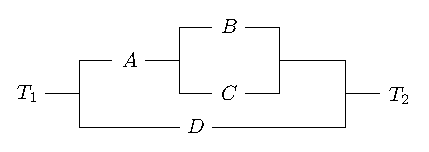
\includegraphics[height=20mm]{vezje.eps}
\caption{An example of a circuit with four switches}\label{fig:vezje}
\end{center}
\end{figure}

Suppose that we have such a circuit and we know which switches are open and which ones are closed.
We would like to determine whether the whole circuit is ``closed'' (that is, admits the flow of current)
or ``open'' (no current).

\medskip
First, let us consider two very simple circuits:

(1) {\em two switches connected in series:}
\begin{figure}[h!]
\begin{center}
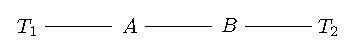
\includegraphics[height=5mm]{vezje-zaporedno.eps}\label{fig:vezje-zap}
\end{center}
\end{figure}

A series circuit is closed if and only if both switches are closed: \textbf{ conjunction}.

(2) {\em two switches connected in parallel:}

\begin{figure}[h!]
\begin{center}
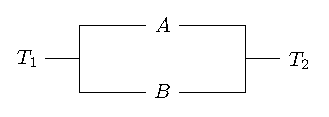
\includegraphics[height=20mm]{vezje-vzporedno.eps}\label{fig:vezje-vzp}
\end{center}
\end{figure}

A parallel circuit is closed if and only if at least one of the two switches is closed: \textbf{ disjunction}.

\medskip
To every such circuit we can associate a logical proposition, composed of propositions corresponding to switches.

\medskip
And conversely: by means of {\em identical} and {\em opposite} switches we can represent every
compound proposition with a circuit!

A pair of switches are said to be identical if they are either simultaneously both open or both closed.

A pair of switches are said to be opposite if exactly one of them is open.

\medskip
The following connection between propositions and switches holds:
{\em a circuit  is closed if and only if the corresponding proposition is true, and open otherwise.}

%% 4. predavanje, 2 uri, 12. 10. 2011

\medskip
\paragraph{Example.}
Consider the following proposition:
$$(A\sledi B) \inn (B\sledi C) \inn (\neg A \ali C)$$
We computed its truth table in Chapter $1.2$:
$$\begin{tabular}{c|c|c|c|c}
  \hline
  % after \\: \hline or \cline{col1-col2} \cline{col3-col4} ...
   & $A$ & $B$ & $C$&$(A\sledi B) \inn (B\sledi C) \inn (\neg A \ali C)$\\
  \hline
  1. & 1& 1& 1 & 1 \\
  2. & 1& 1& 0 & 0 \\
  3. & 1& 0& 1 & 0 \\
  4. & 1& 0& 0 & 0 \\
  5. & 0& 1& 1 & 1 \\
  6. & 0& 1& 0 & 0 \\
  7. & 0& 0& 1 & 1 \\
  8. & 0& 0& 0 & 1 \\
\end{tabular}$$
In the previous chapter we wrote this proposition in its canonical DNF as:
$$(A\inn B\inn C) \ali (\neg A\inn B\inn C)\ali (\neg A\inn \neg B\inn C)\ali (\neg A\inn \neg B\inn \neg C)\,.$$

This form corresponds to the following circuit:
\begin{figure}[h!]
\begin{center}
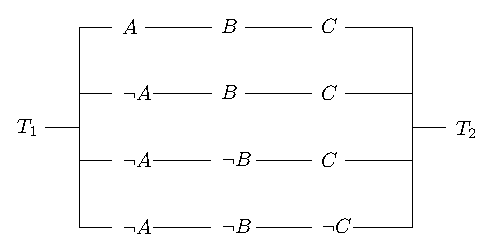
\includegraphics[height=35mm]{vezje-DNO.eps}\label{fig:vezje-DNO}
\end{center}
\end{figure}

On the other hand, the canonical CNF
$$(\neg A\ali\neg B \ali C) \inn (\neg A\ali B \ali \neg C)\inn
(\neg A\ali B \ali C) \inn (A\ali \neg B \ali C)$$
corresponds to circuit
\begin{figure}[h]
\begin{center}
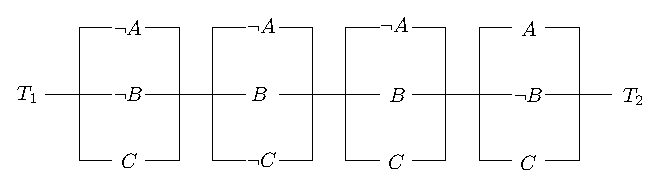
\includegraphics[height=20mm]{vezje-KNO.eps}\label{fig:vezje-KNO}
\end{center}
\end{figure}

Therefore, a single proposition can be represented by more than one switching circuit.
It is therefore reasonable to require that, in the actual physical
construction of circuits simulating a given proposition, our goal is to find a
circuit as simple as possible. Perhaps the circuit should also satisfy certain other requirements
(depending on the application). We will not consider these issues here.
\kz

\bigskip
\paragraph{Example.}
Consider the following switching circuit:

\begin{figure}[h!]
\begin{center}
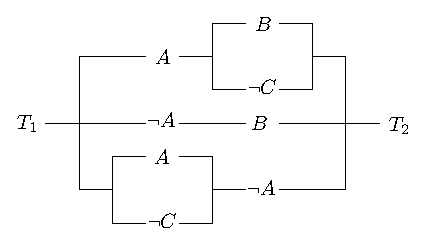
\includegraphics[height=35mm]{vezje2.eps}\label{fig:vezje2}
\end{center}
\end{figure}

{\em For which switch positions is the circuit closed?}

Let us solve the problem with logic.

The corresponding proposition, say $D$, is:
$$(A \inn B\ali \neg C)\ali (\neg A \inn B)\ali (A \ali \neg C \inn \neg A)\,.$$
Its truth table is:
$$\begin{tabular}{c|c|c|c|c|c|c|c}
  \hline
  % after \\: \hline or \cline{col1-col2} \cline{col3-col4} ...
   & $A$ & $B$ & $C$ & $A \inn B\ali \neg C$ & $\neg A \inn B$ & $A \ali \neg C \inn \neg A$ & $D$\\
  \hline
  1. & 1 & 1 & 1 & 1 & 0 & 0 & 1\\
  2. & 1 & 1 & 0 & 1 & 0 & 0 & 1\\
  3. & 1 & 0 & 1 & 0 & 0 & 0 & 0\\
  4. & 1 & 0 & 0 & 1 & 0 & 0 & 1\\
  5. & 0 & 1 & 1 & 0 & 1 & 0 & 1\\
  6. & 0 & 1 & 0 & 0 & 1 & 1 & 1\\
  7. & 0 & 0 & 1 & 0 & 0 & 0 & 0\\
  8. & 0 & 0 & 0 & 0 & 0 & 1 & 1\\
\end{tabular}$$
We see that the circuit is open if and only if switch $B$ is open and switch $C$ is closed, and closed in all other cases.

Hence, we could replace the circuit with the following simpler one:
\begin{figure}[h!]
\begin{center}
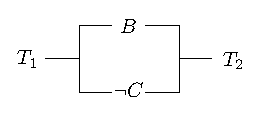
\includegraphics[height=15mm]{vezje3.eps}\label{fig:vezje3}
\end{center}
\end{figure}

The same result could be derived in a purely logical way:

From the truth table, we read off the canonical CNF of $D$:
$$(\neg A \ali B \ali \neg C) \inn (A \ali B\ali \neg C)\,.$$
Using distributivity, we see that this proposition is equivalent to the following one:
$$(\neg A \ali \inn A) \ali (B\ali \neg C)\,,$$
however, since the conjunction $\neg A \ali \inn A$ is always false, the above proposition is equivalent to
the proposition
$$B\ali \neg C\,.$$\kz

\medskip
We conclude this chapter with a more practical example.

\medskip
\paragraph{Example.}
Consider a committee of $3$ members voting about individual motions according to a certain voting rule.
The task is to construct a switching circuit that would tell immediately
whether the motion is accepted or not.

Let us consider the following two voting rules:

(a) the principle of simple majority

(b) the principle of simple majority, where member $A$ has a right to veto

The truth table says:
$$\begin{tabular}{c|c|c|c|c}
  \hline
  % after \\: \hline or \cline{col1-col2} \cline{col3-col4} ...
$A$ & $B$ & $C$  & $(a)$ & (b)\\
  \hline
1 & 1 & 1 & 1  & 1  \\
1 & 1 & 0 & 1  & 1  \\
1 & 0 & 1 & 1  & 1  \\
1 & 0 & 0 & 0  & 0  \\
0 & 1 & 1 & 1  & 0  \\
0 & 1 & 0 & 0  & 0  \\
0 & 0 & 1 & 0  & 0  \\
0 & 0 & 0 & 0  & 0  \\
\end{tabular}$$

The canonical DNF of the sought proposition in case (a) reads
$$(A\inn B\inn C)\ali (A\inn B\inn \neg C)\ali (A\inn \neg B\inn C)\ali (\neg A\inn B\inn C)$$
and in case (b)
$$(A\inn B\inn C)\ali (A\inn B\inn \neg C)\ali (A\inn \neg B\inn C)\,.$$
The corresponding circuits are depicted on Figure~\ref{fig:comittee}.
\kz
\begin{figure}[htbp]
	\begin{center}
		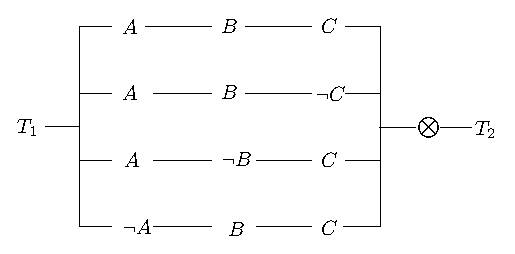
\includegraphics[height=30mm]{vezje-poslanci-1.eps} \\ \vspace{0.5cm}
		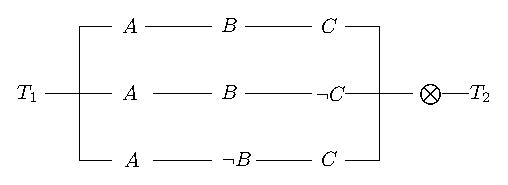
\includegraphics[height=20mm]{vezje-poslanci-2.eps}
	\end{center}
	\caption{\label{fig:comittee} The corresponding circuits for the comittee (a) withouth a veto member (above), and (b) with veto for the member $A$ (below).}
\end{figure}
%\textbf{ Homework:} Construct a circuit that simulates the proposition
%$$(A\sledi B) \ali (\neg B\sledi C) \ali (A \cee C)\,.$$

\section{Logical implications}

A {\em logical implication} is a tautology such that the main connective is an implication.
It $B\sledi C$ is a tautology, then the truth subspace of the antecedent (that is, proposition $B$) is
 contained in the truth subspace of the consequent (that is, proposition $C$). And conversely,
 if the truth subspace of the antecedent is contained in the truth subspace of the consequent, then
$B\sledi C$ is a tautology.

\textbf{ Homework:} Prove the statement that $B\sledi C$ is a tautology if and only if
the truth subspace of the antecedent is contained in the truth subspace of the consequent.

\bigskip
The following basic facts about logical implications hold:
\begin{enumerate}
  \item If the antecedent is a tautology, then also the consequent is a
  tautology.
  \item If the consequent is a contradiction, then also the antecedent is a contradiction.
  \item If the consequent is a tautology, then the antecedent can be any proposition.
  \item If the antecedent is a contradiction, then the consequent can be any proposition.
  \item Every proposition logically implies itself.
  \item Every proposition that logically implies both some proposition $A$ and its negation $\neg A$, must be a contradiction.
  \item Every proposition that logically implies its own negation, is a contradiction.
\end{enumerate}


\textbf{ Some comments to the implications:}

(1.) From the truthfulness of the antecedent and the truth of the implication we can infer the truth of the consequent.
\begin{itemize}
  \item In classical logic this inference rule was called {\em mixed hypothetical syllogism}, namely {\em modus ponendo ponens} (lat.~the way that affirmes by affirming).
\end{itemize}

\paragraph{Example.}
\begin{itemize}
    \item If today is Monday, I will go to the lectures.
    \item Today is Monday.
    \item[$\circ$] \textbf{Conclusion:} I will go to the lectures.\kz
\end{itemize}


\medskip

(2.) {\em mixed hypothetical syllogism} {\em modus tollendo tollens} (lat.~the way that denies by denying)

\textbf{ Examples:}

1. Where there is smoke, there is also fire.

Here there is no fire.

Conclusion: Here there is no smoke.

2. A person that is happy with little lives well.

A greedy person does not live well.

Conclusion: A greedy person is not happy with little.


(3.) {\em disjunctive syllogism} {\em modus tollendo ponens}
(lat.~the way that affirms by denying)


\medskip
\textbf{ Example:}

Koper is a country or it is a town.

Koper is not a country.

Conclusion: Koper is a town.

(4.) Simplification.

(5.) Addition.

(6.) From a contradiction an arbitrary proposition can be derived.

(7.) Transitivity of implication (so called~{\em pure hypothetical syllogism}).

(12.) Transitivity of equivalence.

(19.) The rule of absurd.

\subsubsection*{Some important logical implications}

\begin{enumerate}
	\item $A \inn (A \sledi B) \sledi B$
	\item $\neg B \inn (A \sledi B) \sledi \neg A$
	\item $\neg A \inn (A \ali B) \sledi B$
	\item $A \inn B \sledi A$
	\item $A \sledi A\ali B$
	\item $A \inn \neg A\sledi B$
	\item $(A \sledi B) \inn (B \sledi C) \sledi (A\sledi C)$
	\item $(A \sledi B) \sledi (C \sledi A \sledi (C\sledi B))$
	\item $(A \sledi B) \sledi (B \sledi C \sledi (A\sledi C))$
	\item $(A \sledi B) \sledi (A\inn C \sledi B\inn C)$
	\item $(A \sledi B) \sledi (A\ali C \sledi B\ali C)$
	\item $(A \cee B) \inn (B\cee C) \sledi (A\cee C)$
	\item $(A \cee B) \sledi (A\sledi B)$
	\item $(A \cee B) \sledi (B\sledi A)$
	\item $A \inn (A \cee B) \sledi B$
	\item $\neg A \inn (A \cee B) \sledi \neg B$
	\item $B\sledi (A\cee A \inn B)$
	\item $\neg B\sledi (A\cee A \ali B)$
	\item $(A\sledi (B\inn \neg B)) \sledi \neg A$
\end{enumerate}

As an exercise, convince yourself in the validity of these logical implications.
Instead of truth tables, you may use the following method: {\em Starting from the definition of a logical implication, try to construct such a truth assignment for which the implication is false. Of course, it then has to turn out that such a truth assignment does not exist.}

\bigskip
\paragraph{Example.}
Let us prove the $10$th implication from the list:
$$A \sledi B \sledi (A\inn C \sledi B\inn C)$$
This implication would only be false for a truth assignment for which the proposition
$A \sledi B$ would be true, while the proposition $A\inn C \sledi B\inn C$ would be false.
However, according to the definition of the implication, this is true only if the propositions
$A$ and $C$ are true, while proposition $B$ is false.
In this case the implication $A \sledi B$ is false, which contradicts the assumption that it is true.
Therefore, an assignment for which the proposition $A \sledi B$ would be true and the proposition $A\inn C \sledi B\inn C$ false, does not exist.
Implication $10$ is indeed a tautology.\kz
\medskip



\section{Proofs}
Here we describe several types of proofs.
\subsection{Direct proof}

We would like to prove the truthfulness of logical implication $A \sledi  B$.
We assume that proposition $A$ is true, and directly derive the truthfulness of proposition $B$.


\medskip
\textbf{ Example:}
If $n$ is an odd natural number, then also $n^2$ is odd.

Proof: Let $n$ be an odd natural number.
Then we can write it as $n = 2k-1$ for some natural number $k$.
Therefore $n^2 = (2k-1)^2 = 4k^2-4k+1 = 2(2k^2-2k)+1$, hence  $n^2$ is odd. \qed

\subsection{Indirect proof.}

We would like to prove the truthfulness of  logical implication $A \sledi  B$. It is sometimes more convenient to
prove instead equivalent implication $\neg B \sledi \neg A$.

\medskip
\textbf{ Example :} If  $n^2$ is even, then $n$ is also even.

Proof: The proposition is equivalent to the implication:

If $n$ is a number that is not even, then also $n^2$ is a number that is not even.

Equivalently: If $n$ is odd, then also $n^2$ is odd.

But this we just proved.\qed

\subsection{Proof by contradiction.}

We would like to prove the truthfulness of proposition $A$.
We assume that $A$ is false and show that this assumption leads to a contradiction (which we denote by $\perp$).
This way, we showed the truthfulness of the proposition $\neg A \sledi \perp$. But this proposition is only true if proposition $\neg A$ is false. Hence $A$ is true.

\medskip
\textbf{ Example:} $\sqrt 2$ is not rational.

Proof: Suppose that $\sqrt 2$ is a rational number. Then we can write it as $\sqrt 2 = p/q$, where $p$ and $q$ are
two relatively prime natural numbers.

It follows that

$2 = p^2/q^2$.

$p^2 = 2q^2$.

Hence $p^2$ is even. Therefore (according to what we proved above) $p$ is even.

Let us write $p = 2m$, where $m$ is a natural number.

We obtain

$4m^2 = 2q^2$.

Thus
$2m^2 = q^2$.

Hence, also $q$ is even. This, however, is a contradiction. (We assumed that $p$ and $q$ are relatively prime numbers and showed that they are both divisible by $2$.)\qed




\subsection{Propositions with quantifiers}
Quantifiers tell, for  how many objects of some kind a given proposition is true.
We will use the following notation:

%$\forall$... za vsak
%
%$\exists$ ... obstaja (s tujko: eksistira)
%
%$\exists!$ ... obstaja natanko eden.
%
\begin{itemize}
  \item
  $(\forall x) A(x)$ ... for every $x$ proposition $A(x)$ is true.
  \item
  $(\exists  x) A(x)$ ... there exists an $x$ such that proposition $A(x)$ is true.
  \item
  $(\exists!  x) A(x)$ ... there exists a unique (that is, one and only one) $x$ such that proposition $A(x)$ is true.
\end{itemize}

\medskip
\textbf{ Examples:}
\begin{itemize}
  \item
$(\forall$ natural numbers $n)$ ($n$ is divisible by $2$).
  \item
$(\exists n)$ ($n$ is a natural number and $n$ is divisible by $2$).
  \item
$(\exists !n)$ ($n$ is the smallest natural number).
\end{itemize}

\subsubsection{Negation of propositions with quantifiers}

\textbf{ Negation $\forall$}
$$\neg (\forall x)A(x) \cee  (\exists x) (\neg A(x))$$

\medskip
\paragraph{Example.}

$B$: Every citizen of Slovenia is dark haired.

$\neg B$: It is not true that every citizen of Slovenia is dark haired.

Equivalently: There exists at least one citizen of Slovenia that is not dark haired.\kz

\medskip

\noindent\textbf{ Negation $\exists$}
$$\neg  (\exists x)A(x) \cee (\forall x) \neg A(x)$$

\medskip
\paragraph{Example.}

$B$: There is a red ball in the box.

$\neg B$: It is not true that there is a red ball in the box.

Equivalently: For every ball in the box, it holds that it is not red.\kz


\medskip

\noindent\textbf{ Negation $\exists !$}
$$\neg (\exists ! x)A(x) \cee  (\forall x) (\neg A(x)) \ali (\exists x)(\exists y)(x\neq y\inn A(x) \inn A(y))$$

\medskip
\paragraph{Example.}

$B$: There exists a unique prime number.

$\neg B$: It is not true that there exists a unique prime number.

Equivalently: Either no number is prime, or there exists at least two different prime numbers.\kz

\bigskip
\paragraph{Example.}

Is the following proposition correct?

There exists a real number $x$ such that $\frac{1}{1+x^2}>1$.

$$(\exists x) (\frac{1}{1+x^2} > 1)$$

No, the proposition is not true. We can check that its negation is true:
$$\neg (\exists x) (\frac{1}{1+x^2} > 1)$$
$$\cee (\forall x) \neg (\frac{1}{1+x^2} > 1)$$
$$\cee (\forall x) (\frac{1}{1+x^2} \le  1)$$
$$\cee (\forall x) (1 \le  1+x^2)$$
$$\cee (\forall x) (0 \le  x^2)$$

Hence:

$$
\neg  \left(
\exists \,\mathrm{ real \, number }\,x: \frac{1}{x^2+1}>1
\right)
$$\kz


\medskip
\paragraph{Example.}

Let $P(x)$ denote the proposition ``$x$ is prime''.

{\emph For every natural number $x$ there exists a natural number $y$, bigger than $x$, that is a prime number:
  $(\forall x)(\exists y)(y>x\inn P(y))$.}

  Negation:   $$\neg (\forall x)(\exists y)(y>x\inn P(y)) \cee(\exists  x)\neg (\exists y)(y>x\inn P(y))$$
  $$\cee(\exists  x)(\forall  y)\neg (y>x\inn P(y))\cee(\exists  x)(\forall  y)(y\le x\ali \neg P(y))\,.$$


\bigskip
\bigskip
\paragraph{Example.}
Let us write the negation of the proposition
  $$(\forall x)(\exists y)(y<x)\,.$$

  $$\neg(\forall x)(\exists y)(y<x)$$
  $$\cee$$
  $$(\exists x)(\neg(\exists y)(y<x))$$
  $$\cee$$
  $$(\exists x)(\forall y)\neg(y<x)$$
  $$\cee$$
  $$(\exists x)(\forall y)(y\ge x)$$\kz

\begin{itemize}
  \item Is the following proposition true in real numbers?
  $$(\forall x)(\exists y)(y<x)$$
  Yes, the proposition is true!

  \item Is it true in natural numbers?
  $$(\forall x)(\exists y)(y<x)$$

No, its negation is true:
$$(\exists x)(\forall y)(y\ge x)\,,$$
since there exists a smallest natural number.
\end{itemize}
%end of lecture 3
\subsection*{Inference of Propositions}

\begin{center}
\begin{tabular}{|c|c|c|}
	\hline 
	name & assumption(s) & conclusion\\
	\hline 
	\hline 
	modus ponens & $A,A\Rightarrow B$ & $B$\\
	\hline 
	modus tollens & $A\Rightarrow B,\neg B$ & $\neg A$\\
	\hline 
	hipoteti\v{c}ni silogizem & $A\Rightarrow B,B\Rightarrow C$ & $A\Rightarrow C$\\
	\hline 
	disjunktivni silogizem & $A\vee B,\neg A$ & $B$\\
	\hline 
	združitev  & $A,B$ & $A\wedge B$\\
	\hline 
	poenostavitev & $A\wedge B$ & $A$\\
	\hline 
	pridružitev & $A$ & $A\vee B$\\
	\hline 
\end{tabular}
\end{center}

\textbf{Example 1}:
\begin{itemize}
	\item I will go to the match.
	\item In the evening, I will do the homework.
	\item If I go to the match and then to the cinema, I will not have the time to do the homework.
\end{itemize}
Can I infer that I will not be able to go to the cinema?

\medskip
\textbf{ Solution:}

Let us define the following propositions:

$A_1$: I will go to the match.

$A_2$: In the evening, I will do the homework.

$A_3$: I will go to the cinema.

$C_1$: $A_1$

$C_2$: $A_2$

$C_3$: $A_1\inn A_3\sledi \neg A_2$.

We have to determine whether the implication
$$C_1\inn C_2\inn C_3\sledi \neg A_3$$
is a tautology.

\textbf{Example 2}

The following facts are given:
\begin{itemize}
	\item This animal is not a bird, or it has wings.
	\item If this animal is a bird, then it lays eggs.
\end{itemize}
Is the following inference correct?
{\em If this animal does not have wings, then it does not lay eggs.}

\medskip
\textbf{ Solution:}

Let us define the following propositions:

$A_1$: This animal is a bird.

$A_2$: This animal has wings.

$A_3$: This animal lays eggs.

$C_1$: $\neg A_1\ali A_2$

$C_2$: $A_1\sledi A_3$

$B$: $\neg A_2\sledi \neg A_3$.

We have to determine whether the implication
$$C_1\inn C_2\sledi B$$
is a tautology.

\subsection{Sets of propositions}

We are given atomic propositions $A_1,\ldots, A_n$ (that is, propositions without any logical connectives).

How many different propositions can we built out of them?

It seems that infinitely many! However, for logic, two propositions are the same if they are logically equivalent.

There are only finitely many propositions that are pairwise logically non-equivalent!

The assignment space of every proposition composed of $A_1,\ldots, A_n$, consists of exactly $2^n$ different truth assignments.
A proposition is uniquely defined (up to logical equivalence), as soon as we define its values for each of these $2^n$ truth assignments.

Every truth assignment takes one of the two values $0$ and $1$, independently of the others.
Consequently, the number of possible propositions is
$2^{(2^n)}$.

\bigskip
Let us examine the construction of all possible propositions for $n = 1$ and $n=2$.

\textbf{ n = 1}

We have only one atomic proposition $A$. From it, we can build $2^{(2^1)} = 4$ propositions, $C_1,\ldots, C_4$.

$$\begin{tabular}{c|c|c|c|c}
\hline
% after \\: \hline or \cline{col1-col2} \cline{col3-col4} ...
$A$ & $C_1$ & $C_2$  & $C_3$ & $C_4$\\
\hline
1 & 1 & 1 & 0  & 0  \\
0 & 1 & 0 & 1  & 0  \\
\end{tabular}$$

$C_1$ is the tautology, e.g.~$A\ali \neg A$.

$C_4$ is the contradiction, e.g.~$A\inn \neg A$.

For $C_2$ we can take just $A$.

For  $C_3$ we can take  $\neg A$.


\bigskip
\textbf{ n = 2}

We have two propositions, $A$ and $B$. From them, we can build $2^{(2^2)} = 16$ propositions,
$C_1,\ldots, C_{16}$.

$$
\begin{tabular}{c|c|c|c|c|c|c|c|c|c}
\hline
$A$ & $B$
& $C_1$ & $C_2$  & $C_3$ & $C_4$
& $C_5$ & $C_6$  & $C_7$ & $C_8$\\
\hline
1 & 1 & 1 & 1 & 1 & 1 & 1 & 1 & 1 & 1\\
1 & 0 & 1 & 1 & 1 & 1 & 0 & 0 & 0 & 0\\
0 & 1 & 1 & 1 & 0 & 0 & 1 & 1 & 0 & 0\\
0 & 0 & 1 & 0 & 1 & 0 & 1 & 0 & 1 & 0\\
\hline
\hline
$A$ & $B$
& $C_9$ & $C_{10}$  & $C_{11}$ & $C_{12}$
& $C_{13}$ & $C_{14}$  & $C_{15}$ & $C_{16}$\\
\hline
1 & 1 & 0 & 0 & 0 & 0 & 0 & 0 & 0 & 0\\
1 & 0 & 1 & 1 & 1 & 1 & 0 & 0 & 0 & 0\\
0 & 1 & 1 & 1 & 0 & 0 & 1 & 1 & 0 & 0\\
0 & 0 & 1 & 0 & 1 & 0 & 1 & 0 & 1 & 0\\
\end{tabular}
$$

Of course, $C_1$ is the tautology, e.g.,~$A\ali \neg A$, and
$C_{16}$ is the contradiction $A\inn \neg A$.

Propositions $C_2$, $C_3$, $C_5$ and $C_9$ are only false for one truth assignment, hence we can express them with the canonical
CNF:
\begin{itemize}
	\item $C_2 = A\ali B$
	\item $C_3 = A\ali \neg B$
	\item $C_5 = \neg A\ali B$
	\item $C_8 = \neg A\ali \neg B$
\end{itemize}
Similarly, the propositions $C_{8}$, $C_{12}$, $C_{14}$ and $C_{15}$ can be expressed with their canonical DNF:
\begin{itemize}
	\item $C_8 = A\inn B$
	\item $C_{12} = A\inn\neg B$
	\item $C_{14} = \neg A\inn B$
	\item $C_{15} = \neg A\inn\neg B$
\end{itemize}
Each of the remaining propositions is true for two truth assignments, and also false for two truth assignments.

For $C_4$ we can take $$(A\inn B) \ali (A\inn \neg B)\,,$$
which is equivalent to
$$A\inn B \ali \neg B$$
and since the disjunction $B \ali \neg B$ is always true, proposition $C_4$ is equivalent to proposition $A$.

Similarly, we can verify that:
\begin{itemize}
	\item  proposition $C_6$ is equivalent to proposition $B$,
	\item  proposition $C_{11}$ is equivalent to proposition $\neg B$,
	\item  proposition $C_{13}$ is equivalent to proposition $\neg A$.
\end{itemize}
For $C_7$ let us write
$$(A\inn B) \ali (\neg A\ali \neg B)\,,$$
which is equivalent to
$$A\cee B\,.$$
Similarly, for $C_{10}$ we can take the equivalence
$$A\cee \neg B\,.$$
\qed


\section{Exercises}

\textbf{ 1.}
The following two propositions are given:
$A$: ``Andrej speaks French.'' and $B$: ``Andrej speaks Danish.''
Write the following compound propositions in natural language:

(a) $A\ali B$

(b) $A\inn B$

(c) $A\inn \neg B$

(d) $\neg A\ali \neg B$

(e) $\neg \neg A$

(f) $\neg (\neg A\inn \neg B)$

\medskip
\textbf{ 2.}
The following two propositions are given:
$A$: ``Janez is rich.'' and $B$: ``Janez is happy.''

Write the following propositions symbolically:

(a) If Janez is rich, then he is unhappy.

(b) Janez is neither happy nor rich.

(c) Janez is happy only if he is poor.

(d) Janez is poor if and only if he is unhappy.

\textbf{ Exercise:} Solve the following exercises about knights and servants:
\begin{itemize}
  \item Arthur: ``It is not true that Bine is a servant."~Bine: ``We are not both of the same kind.''
  \item Arthur: ``It is not true that Cene is servant."~Bine: ``Cene is a knight or I am a knight."~Cene: ``Bine is a servant."
\end{itemize}

\textbf{ A similar exercise:}
Now Arthur and Bine say the following:
\begin{itemize}
 \item Arthur: ``Me and Bine are not of the same kind.''
 \item Bine: ``Exactly one of us is a knight.''
\end{itemize}
\chapter{Set Theory}

\section{Sets}

Elements (objects): $a,b,\ldots, x,y,z$ (+ indices: $a_6, x_1, z_\lambda$)

Sets: $A,B,\ldots, X,Y,Z$ (+ indices)

$a\in F$: element $a$ belongs to set $F$, $a$ is an element of set $F$.

$\in$: symbol of containment

$a\not\in F$: $a$ is not an element of (does not belong to) set $F$.

\textbf{ Example:}
If $G$ is the set of all even numbers, then $16\in G$ and $3\not\in G$.


\medskip
{\em Equality of sets:} Sets $A$ and $B$ are equal if and only if they have exactly the same objects as elements:

$$A = B \cee (\forall x) (x\in A\cee x\in B)$$

\medskip
This definition is necessary, since it describes an important property that the containment relation must satisfy!

\medskip

\textbf{ Example:} Suppose that the objects under consideration are people, and
let us write $x\in A$ if and only if $x$ is an ancestor of  $A$.
Can we use this definition to define people as sets?
The above equivalence says:
\begin{itemize}
  \item {\em If two people are the same then they have the same ancestors.} This is true.
  \item {\em If two people have the same ancestors, then they are the same.} This however is not true!
\end{itemize}

\bigskip
A set can be given by a list of all its elements:
$$A = \left\{1,\frac{1}{2}, \frac{\pi}{3}, 2i+8\right\}\,.$$
The order {\em is irrelevant!}

\medskip
Sometimes such a description is impractical:
\begin{itemize}
  \item If the set is infinite (e.g., the set of all prime numbers).
  \item If the set is finite but too large (e.g., the set of all books that were printed on Planet Earth until the year 2011),
\end{itemize}

\medskip
A set can also be given by a description of it. The description must be unambiguous:
for every object, it must hold that it either belongs to the set, or that it does not belong to the set.

\medskip
\textbf{ Example:} Let $A$ be the set of all complex numbers  $x$ that are a solution of some equation of the form
$$a_nx^n+a_{n-1}x^{n-1}+\cdots+a_1x+a_0 = 0\,,$$
where $n\in \mathbb{N}$ and $a_i\in \mathbb{Z}$ for all $i= 0,1,\ldots, n$.

\medskip
$A$ - the set of all algebraic numbers.

Is $2^{\pi}\in A$? We do not know (contemporary mathematics cannot yet give an answer this question).\qed

\medskip
In general, we can write:
$$A = \{x; P(x)\}\,,$$
{\em set $A$ is the set of all elements $x$ such that proposition $P(x)$ is true.}
Or, if we have several propositions $P_1,\ldots, P_n$:
$$A = \{x; P_1(x)\inn \cdots\inn P_n(x)\}$$
$$A = \{x; P_1(x)\ali \cdots\ali P_n(x)\}$$
As we will see soon, we can build such sets only with elements of the sets that we already know (or for which we know that they exist).

\medskip
\textbf{ Example:}
Let  $L$ be the set of all people. Propositions `$x$ is married''~and ``$x$ is at least 20 years old''~are meaningful for elements of the set $L$.
Hence, we can construct sets
      $$\{x\in L; x \textrm{ is married}\}$$
      $$\{x\in L; x \textrm{ is married} \inn x \textrm{ is at least 20 years old}\}$$
as well as (by negating the above conjunction)
      $$\{x\in L; x \textrm{ is not married} \ali x \textrm{ is not at least 20 years old}\}$$

The set
      $$\{x\in L; x \textrm{ is the current president of Republic of Slovenia}\}$$
contains only Borut Pahor and nothing else.

\medskip
Be careful: a box that contains a hat is not the same thing as the hat.
Similarly, the set
$\{a\}$ is not the same thing as $a$. For every object $a$, it holds that $a\in \{a\}$.

\section{Empty set}
We denote the set that has no elements with symbol $\emptyset$ --- {\em empty set}.

$$X = \emptyset \cee (\forall x)(x\not\in X)$$

Of course it holds that:
$$(\forall X) (\emptyset \subseteq X)$$

\section{Subsets}
We are given two sets $A$ and $B$.

We say that $A$ is a {\em subset} of $B$ if and only if every element of $A$ is also an element of  $B$.

Notation: $A\subseteq B$

$$A\subseteq B\cee (\forall x)(x\in A\sledi x\in B)$$

Of course, every set is a subset of itself: $$(\forall A)(A\subseteq A)\,.$$

If $A\subseteq B$ and $A\neq B$, then $A$ is a  {\em proper subset } of set $B$: $A\subset B$.

$$A\subset B\cee (A\subseteq B \inn A\neq B)$$

Clearly, it holds that:
\begin{itemize}
  \item $A\subseteq B \inn B\subseteq A \cee A = B$.

  This equivalence is extremely important for proving equality of two sets!
  \item $A\subseteq B \inn B\subseteq C \sledi A \subseteq C \textrm{~(transitivity of inclusion)}$
\end{itemize}

For our proof of equivalence $A\subseteq B \inn B\subseteq A \cee A = B$, we will need the following
equivalence:
$$(\forall x)(P(x)\inn Q(x))\cee (\forall x)P(x)\inn (\forall x)Q(x)\,.$$

Proof:

$(\Rightarrow)$:

Proof by contradiction.
Suppose that $(\forall x)(P(x)\inn Q(x))$, while

$\neg((\forall x)P(x)\inn (\forall x)Q(x))\,.$

Then:
$\neg(\forall x)P(x)\ali \neg (\forall x)Q(x)\,.$

$(\exists  x)\neg P(x)\ali (\exists x)\neg Q(x)\,.$

Independently of which of the propositions $(\exists  x)\neg P(x)$
and $(\exists  x)\neg Q(x)$ is true, we have a contradiction with proposition
$(\forall x)(P(x)\inn Q(x))$.

$(\Leftarrow)$:

Proof by contradiction.
Suppose that $(\forall x)P(x)\inn (\forall x)Q(x)\,,$ while

$\neg (\forall x)(P(x)\inn Q(x))$.

Then:
$(\exists  x)\neg (P(x)\inn Q(x))$.

$(\exists  x)(\neg P(x)\ali \neg Q(x))$.

Choose $x$ such that $\neg P(x)\ali \neg Q(x)$.

Independently of which of the propositions $\neg P(x)$ and $\neg Q(x)$
is true, we have a contradiction with proposition
$(\forall x)P(x)\inn (\forall x)Q(x)\,.$\qed

\bigskip
Let us now prove the equivalence
$$A\subseteq B \inn B\subseteq A \cee A = B\,:$$

$$A\subseteq B \inn B\subseteq A$$
$$\cee$$
$$(\forall x)(x\in A\sledi x\in B) \inn (\forall x)(x\in B\sledi x\in A)$$
$$\cee$$
$$(\forall x)((x\in A\sledi x\in B) \inn (x\in B\sledi x\in A))$$
$$\cee$$
$$(\forall x)(x\in A\cee x\in B)$$
$$\cee$$
$$A = B\,.$$\qed


\textbf{ Homework:} prove the above implication (transitivity of inclusion).

\medskip
\textbf{ A question:} Do there exist two sets $A$ and $B$ such that $A\subset B$ and $B\subset A$?

\bigskip
\textbf{ Be careful:} relation of inclusion $\subseteq$ and relation of containment $\in$ are two completely different
notions!

$1\in\{1,2,3\}$, but $1$ is not a subset of the set $\{1,2,3\}$.
Set $\{1\}$ is a subset of the set $\{1,2,3\}$, but
$\{1\}$ is not an element of the set $\{1,2,3\}$.

\medskip

\textbf{ Some questions:} Let $X = \{1,2,\{1\},\{2\}\}$.
Is $1$ an element of $X$?
Is $1$ a subset of $X$?
Is $\{1\}$ an element of $X$?
Is $\{1\}$ a subset of $X$?

\bigskip

\section{Union}
We are given two sets $A$ and $B$. The {\em union} of these two sets is the set $A\cup B$,
that has for elements precisely those objects that are elements of the set $A$ or of the set $B$:
$$A\cup B = \{x; x\in A \ali x\in B\}\,.$$

\textbf{ Example:}
$A = \{1,3,5,7\}$, $B = \{1,2,4,8\}$.

$A\cup B = \{1,3,5,7,2,4,8\}$.

\medskip

\textbf{ Union of several sets}:

${\cal A} = \{A_\lambda; \lambda \in J\}$ - union of sets with index set $J$

The index set can be an arbitrary set!

We define the union of an arbitrary family of sets as
$$\cup {\cal A} = \cup_{\lambda \in J} A_\lambda = \{x;(\exists \lambda) (\lambda \in J\inn x\in A_\lambda)\}$$

\medskip
\textbf{ Example:} $J = \{1,2\}$
$$\cup_{\lambda \in \{1,2\}} A_\lambda = \{x;(\exists \lambda) (\lambda \in \{1,2\}\inn x\in A_\lambda)\}= \{x;x\in A_1 \ali x\in A_2\} = A_1\cup A_2\,.$$

\medskip
If $J$ is finite, we usually take $J = \{1,2,\ldots, n\}$ and write
$$\cup {\cal A} = \cup_{j = 1}^nA_j = A_1\cup\cdots\cup A_n\,.$$

\bigskip
\textbf{ Basic properties of the union:}
\begin{itemize}
  \item $A\cup B = B\cup A$, commutativity
  \item $(A\cup B)\cup C = A\cup (B\cup C)$, associativity
  \item $A\cup A = A$, idempotency
  \item $A\cup \emptyset = A$
  \item $A\subseteq A\cup B$, $B\subseteq A\cup B$
  \item $A\subseteq B\cee A\cup B = B$
  \item $A\subseteq C\inn B\subseteq C\sledi A\cup B \subseteq C$
\end{itemize}

\bigskip
Let us prove the property
$$A\subseteq B\cee A\cup B = B\,:$$
\medskip
We will show the equivalence by proving the converse equivalence
$\neg(A\subseteq B)\cee \neg(A\cup B = B)\,:$
$$\neg(A\subseteq B)$$
$$\cee$$
$$\neg(\forall x)(x\in A\sledi x\in B)$$
$$\cee$$
$$(\exists x)(x\in A \inn x\not\in B)$$
$$\cee$$
$$(\exists x)((x\in A \inn x\not\in B) \ali (x\in B \inn x\not\in B))$$
$$\cee$$
$$(\exists x)((x\in A \ali x\in B)\inn x\not\in B)$$
$$\cee$$
$$(\exists x)(x\in A\cup B\inn x\not\in B)$$
$$\cee$$
$$\neg(A\cup B \subseteq B)$$
$$\cee$$
$$\neg(A\cup B \subseteq B) \ali \neg(B \subseteq A\cup B) $$
$$\cee$$
$$\neg((A\cup B \subseteq B)\inn (B \subseteq A\cup B))$$
$$\cee$$
$$\neg(A\cup B = B)$$
\qed

\bigskip
\textbf{ Homework:} Prove the remaining properties.

\bigskip

%\subsection*{Ponovitev:}
%Zadnjiè smo zaèeli z obravnavo množic.
%
%Relaciji pripadnosti $\in$ and inkluzije $\subseteq$. Podmnožica, prazna set, Russellova antinomija, urejeni par, unija.
%
%\medskip
%Relaciji pripadnosti and inkluzije sta povezani takole:
%$$(\forall x)(\forall X)(x\in X\cee \{x\}\subseteq X)\,.$$
%
%$\{a\}\cup \{\{a\}\} = \{a,\{a\}\}$
%
%$\{a\}\cup \{b\} = \{a,b\}\neq \{\{a\},\{b\}\}$
%
%$\{a\}\cup \{b\}\cup \{c\} = \{a,b,c\}$
%
%Unijo družine množic ${\cal A} = \{A_\lambda; \lambda \in J\}$ smo definirali kot
%\hbox{$\cup {\cal A} = \{x;(\exists \lambda) (\lambda \in J\inn x\in A_\lambda)\}$.}
%
%\hbox{$\cap {\cal A} = \{x;(\forall \lambda) (\lambda \in J\sledi x\in A_\lambda)\}$.}
%
%Kaj dobimo v primeru ${\cal A} = \{A_1\}$? $J= \{1\}$.
%$$\cup \{A_1\}
%= \{x;(\exists \lambda) (\lambda \in \{1\}\inn x\in A_\lambda)\}
%= \{x;(\exists \lambda) (\lambda = 1 \inn x\in A_\lambda)\}
% = \{x;x\in A_1\} = A_1\,.$$
%$$\cap \{A_1\} =
%\{x;(\forall \lambda) (\lambda \in \{1\}\sledi x\in A_\lambda)\}
%= \{x;(\lambda= 1\sledi x\in A_\lambda)\}
% = \{x;x\in A_1\} = A_1\,.$$
%
%Pisano brez indeksov: $\cup \{A\} = \cap \{A\} = A$.
%
%Podobno velja tudi $\cup \{\emptyset\} = \cap \{\emptyset\} = \emptyset$ and $\cup \emptyset = \emptyset$.
%
%\bigskip
%Za ogrevanje dokažimo implikacijo
%$$A\subseteq C\inn B\subseteq C\sledi A\cup B \subseteq C\,:$$
%
%Dokaz s contradictionm:
%$$\neg(A\cup B\subseteq C)$$
%$$\cee$$
%$$(\exists x)(x\in A\cup B\inn x\not\in C)$$
%$$\cee$$
%$$(\exists x)((x\in A \ali x\in B)\inn x\not\in C)$$
%$$\cee$$
%$$(\exists x)((x\in A \inn x\not\in C) \ali (x\in B\inn x\not\in C))$$
%$$\cee$$
%$$(\exists x)((x\in A \inn x\not\in C) \ali (x\in B\inn x\not\in C))$$
%$$\cee$$
%$$(\exists x)(x\in A \inn x\not\in C) \ali (\exists x)(x\in B\inn x\not\in C)$$
%$$\cee$$
%$$\neg(\forall x)(x\in A\sledi x\in C)\ali\neg(\forall x)(x\in B\sledi x\in C)$$
%$$\cee$$
%$$\neg(A \subseteq C) \ali \neg(B\subseteq C)$$
%$$\cee$$
%$$\neg(A \subseteq C \inn B\subseteq C)\,.$$
%\qed
%
%Dokazali smo ne samo implikacijo, ampak ekvivalenco
%$$A\subseteq C\inn B\subseteq C\cee A\cup B \subseteq C\,.$$

%\bigskip
%Rešitev domaèe naloge:
%
%Dejstva:
%
%Barona je umoril eden izmed njegovega osebja: kuharica, strežnik or šofer.
%
%Èe je morilka kuharica, je zastrupila hrano.
%
%Èe je morilec šofer, mu je postavil bombo v avto.
%
%Hrana ni bila zastrupljena and strežnik ni morilec.
%
%Sklep: Morilec je šofer.
%
%\bigskip
%
%\textbf{ Rešitev:}
%
%$K$: Morilka je kuharica.
%
%$S$: Morilec je strežnik.
%
%Š: Morilec je šofer.
%
%H: Kuharica je zastrupila hrano.
%
%B: Šofer je postavil bombo v avto.
%
%\medskip
%Ali je naslednja implication tautology?
%
%$(K\ali S\ali$ \v S$)\inn(K\sledi H)\inn($Š$\sledi B)\inn(\neg H\inn \neg S)\sledi $Š
%
%\bigskip
%Recimo, da ni.
%
%(1) $(K\ali S\ali$ \v S$)(d) = 1$
%
%(2) $(K\sledi H)(d) = 1$
%
%(3) (Š$\sledi B)(d) = 1$
%
%(4) $(\neg H\inn \neg S)(d) = 1$
%
%(5) Š$(d) = 0$
%
%Iz (4) sledi:
%
%(5)  $H(d) = S(d) = 0$.
%
%Iz (2) and (5) potem sledi
%
%(6) $K(d) = 0$.
%
%Iz (1), (5) and (6) potem sledi Š$(d) = 1$. contradiction. proposition je tautology  and sklepanje je pravilno.

\section{Intersection}
We are given two sets, $A$ and $B$. The {\em intersection} of these two sets is the set $A\cap B$,
that contains as elements precisely those objects that are elements of set $A$ and of set $B$:
$$A\cap B = \{x; x\in A \inn x\in B\}\,.$$

\textbf{ Example:}
$A = \{1,3,5,7\}$, $B = \{1,2,4,8\}$.

$A\cap B = \{1\}$.

\medskip

\textbf{ Intersection of several sets}:

${\cal A} = \{A_\lambda; \lambda \in J\}$ - a family of sets with index set $J$, $J\neq \emptyset$!

The index set is an arbitrary nonempty set!

We can define the intersection of an arbitrary nonempty family of sets as
$$\cap {\cal A} = \cap_{\lambda \in J} A_\lambda = \{x;(\forall\lambda) (\lambda \in J\sledi x\in A_\lambda)\}$$
(If $J = \emptyset$, we would have $\cap {\cal A}$ = everything. But such a set does not exist.)

\medskip
If $J$ is finite, we usually take $J = \{1,2,\ldots, n\}$ and write
$$\cap {\cal A} = \cap_{j = 1}^nA_j = A_1\cap\cdots\cap A_n\,.$$

If $A\cap B = \emptyset$, we say that the sets $A$ and $B$ are {\em disjoint}.

\bigskip
\textbf{ Basic properties of intersection:}
\begin{itemize}
  \item $A\cap B = B\cap A$, commutativity
  \item $(A\cap B)\cap C = A\cap (B\cap C)$, associativity
  \item $A\cap A = A$, idempotency
  \item $A\cap \emptyset = \emptyset$
  \item $A\cap B\subseteq A$, $A\cap B\subseteq B$,
  \item $A\subseteq B\cee A\cap B = A$
  \item $A\subseteq B\inn A\subseteq C\sledi A \subseteq B\cap C$
\end{itemize}

\bigskip
\textbf{ Homework:} Prove the above properties. (Proofs are similar to the proofs of analogous properties of the union.)

\bigskip
The union and the intersection are related via the distributivity laws:
$$(A\cup B)\cap C = (A\cap C)\cup (B\cap C)$$
$$(A\cap B)\cup C = (A\cup C)\cap (B\cup C)$$

Let us prove the first distributivity law:
$(A\cup B)\cap C = (A\cap C)\cup (B\cap C)$.

{\em How do we show equality of two sets, $X = Y$? There are several possibilities:
\begin{enumerate}
  \item We show the correctness of the proposition $(\forall x)(x\in X\cee x\in Y)$

  OR:
  \item

  \begin{enumerate}
          \item   We show $X\subseteq Y$, that is, the correctness of the proposition $(\forall x)(x\in X\sledi x\in Y)$.
          \item   We also show $Y\subseteq X$, that is, the correctness of the proposition $(\forall x)(x\in Y\sledi x\in X)$.
        \end{enumerate}
\end{enumerate}}
Let's have a look at the first approach:
$$x\in (A\cup B)\cap C$$
$$\cee$$
$$(x\in A\cup B) \inn (x\in C)$$
$$\cee$$
$$(x\in A\ali x\in B) \inn (x\in C)$$
$$\cee$$
$$(x\in A \inn  x\in C)\ali (x\in B \inn  x\in C) $$
$$\cee$$
$$(x\in A \cap C)\ali (x\in B \cap C) $$
$$\cee$$
$$x\in (A \cap C)\cup (B \cap C)\,.$$
Since the above chain of equivalences holds for an arbitrary $x$, the proposition
$$(\forall x)(x\in (A\cup B)\cap C\cee x\in (A \cap C)\cup (B \cap C))$$
is correct. Hence, the sets are equal.
\qed

The distributivity laws also hold more generally, for nonempty set families:
$$(\bigcup_{\lambda\in J}A_\lambda)\cap (\bigcup_{\mu\in K}B_\mu) =
\bigcup_{\lambda\in J, \mu\in K}(A_\lambda\cap B_\mu)\,.$$
$$(\bigcap_{\lambda\in J}A_\lambda)\cup (\bigcap_{\mu\in K}B_\mu) =
\bigcap_{\lambda\in J, \mu\in K}(A_\lambda\cup B_\mu)\,.$$

\medskip
\textbf{ Homework:} Prove that for arbitrary three sets $A$, $B$, $C$ it holds that:
$$(A\cap B)\cup C = A\cap (B\cup C) \cee C\subseteq A\,.$$
(The condition on the right does not depend on $B$!)


\bigskip
\textbf{ Homework solution.}

Let us prove transitivity of inclusion: $A\subseteq B \inn B\subseteq C \sledi A \subseteq C$

{\em Direct proof:}

Assume that $A\subseteq B$ and $B\subseteq C$.
We need to show: $(\forall x)(x\in A\sledi x\in C)$.

Consider an arbitrary $x\in A$.
\begin{itemize}
  \item Since $x\in A$ and $A\subseteq B$, it follows $x\in B$.
  \item Since $x\in B$ and $B\subseteq C$, it follows $x\in C$.
\end{itemize}
Since $x$ was arbitrary, we proved $(\forall x)(x\in A\sledi x\in C)$, that is, $A\subseteq C$.

\bigskip

\section{Set difference}

We are given two sets $A$ and $B$.

The {\em difference}  of sets $A$ and $B$ is the set that contains as elements precisely those objects that are elements of set $A$ but they are not elements of set $B$.
$$A\brez B = \{x; x\in A\inn x\not\in B\}\,.$$

\textbf{ Example:}
Let $A$ be the set of all prime numbers, and $B$ the set of all positive odd numbers.
Then

$A\brez B = \{2\}$ ($2$ is the only even prime)

$B\brez A = \{1,9,15,21,25,\ldots\}$ (the set of all odd numbers that are not primes)

\bigskip

Basic properties:
\begin{itemize}
  \item $A\brez A = \emptyset$

  \item $A\brez (A\cap B) = A\brez B$

  \item $A\cap (A\brez B) = A\brez B$

  \item $A\brez (B\cup C) = (A\brez B)\cap (A\brez C)$

  \item $A\brez (B\cap C) = (A\brez B)\cup (A\brez C)$

  \item $(A\brez B)\cup B = A\cup B$

  \item $(A\cup B)\brez B = A\brez B$

  \item $(A\cap B)\brez B = \emptyset$

  \item $(A\brez B)\cap B = \emptyset$
\end{itemize}

Let us prove the equality $(A\brez B)\cup B = A\cup B$:

$$x\in (A\brez B)\cup B$$
$$\cee$$
$$x\in A\brez B \ali x\in B$$
$$\cee$$
$$(x\in A\inn x\not\in B) \ali x\in B$$
$$\cee$$
$$(x\in A\ali x\in B) \inn (x\not\in B \ali x\in B)$$
$$\cee$$
$$(x\in A\ali x\in B)$$
$$\cee$$
$$x\in A\cup B$$
\qed

\bigskip
\textbf{ Homework:} Prove the remaining properties.

\bigskip
\bigskip

\section{Complement}
Very frequently in mathemathics, we are in the following situation: we are given some
{\em universal set} $S$, and only care about the elements and subsets of $S$.

Let $A\subseteq S$. Then we can define the  {\em complement of set $A$ (relative to $S$)} as:
$$C_SA = \overline A = S\brez A\,.$$
If the set $S$ is not defined, we cannot talk about the complemet:
$\overline \emptyset$ = set of all sets  --- which does not exist (Russell's antinomy)!

\bigskip
\paragraph{Example.}

Let $S = \{0,1,2,3,\ldots\}$ be the set of all natural numbers, and let $A$ be the set of all prime numbers.
Then $\overline A = \{0,1,4,6,8,9,10,12,\ldots\}$.

\kz

\medskip
Properties of the complement:
\begin{itemize}
  \item
$\overline S = \emptyset,~~~~\overline \emptyset = S$

  \item
$\overline{\overline A} = A,~~~A\cup \overline A = S,~~~~A\cap \overline A = \emptyset$

  \item
$A\brez B = A\cap \overline B$

  \item
$A\subseteq B \cee  \overline B \subseteq \overline A$

  \item
$A= B \cee  \overline A = \overline B$

  \item
$\overline{A\cup B} = \overline A\cap \overline B$,~~~$\overline{A\cap B} = \overline A\cup \overline B$ (De Morgan's laws)
\end{itemize}

De Morgan's laws also hold for an arbitrary family of sets ${\cal A} = \{A_\lambda~;~\lambda\in J\}$:
$$\overline{\cup_{\lambda\in J}A_\lambda} = {\cap_{\lambda\in J}\overline A_\lambda}$$
$$\overline{\cap_{\lambda\in J}A_\lambda} = {\cup_{\lambda\in J}\overline A_\lambda}$$

Because of De Morgan's laws, theorems about sets often come in pairs.
If in a given inclusion, equality or equivalence about unions, intersections and complements of  subsets of a certain set we replace each set with its complement, we interchange all union and intersections, and reverse all inclusions, the result is again a valid inclusion, equality or equivalence. This principle is called \textbf{ principle of duality}.

\bigskip
\paragraph{Example.}

The proposition
$$(A\cap B)\cup C = A\cap (B\cup C) \cee C\subseteq A\,.$$
becomes
$$(\overline A\cup \overline B)\cap \overline C = \overline A\cup (\overline B\cap \overline C) \cee \overline A\subseteq \overline C\,,$$
which is equivalent to
$$(A\cup B)\cap C = A\cup (B\cap C) \cee A\subseteq C$$
(after interchanging the roles of sets and their complements).
\kz

%\subsection*{Venn diagrams}

%All relations and operations over subsets of a given universal set can be nicely displayed with so called {\em Venn diagrams}.

%\begin{figure}[ht]
%\begin{center}
%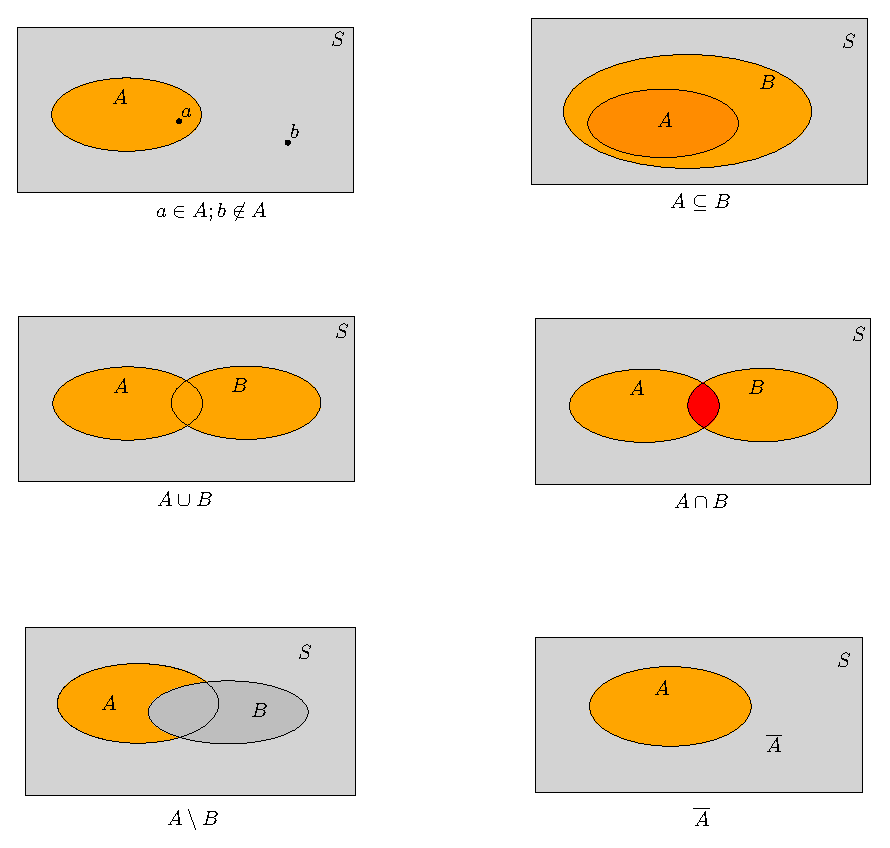
\includegraphics[width=111mm]{Venn.eps}
%\end{center}
%\end{figure}

%$A\subseteq B$:
%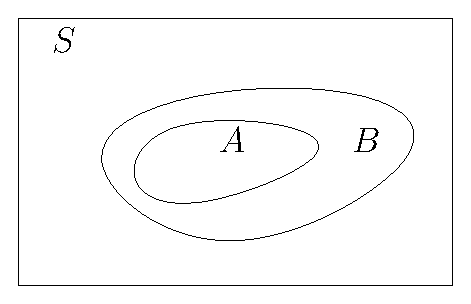
\includegraphics[height=20mm]{diagram1.eps}
%$A\cup B$:
%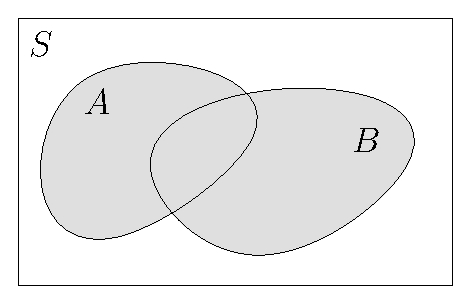
\includegraphics[height=20mm]{diagram2.eps}
%$A\cap B$:
%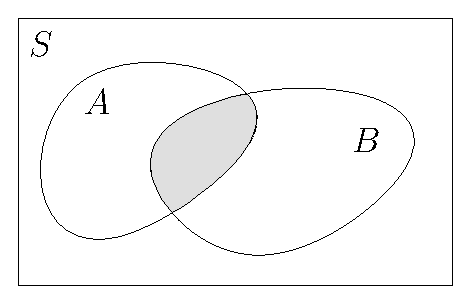
\includegraphics[height=20mm]{diagram3.eps}
%
%$A\brez B$:
%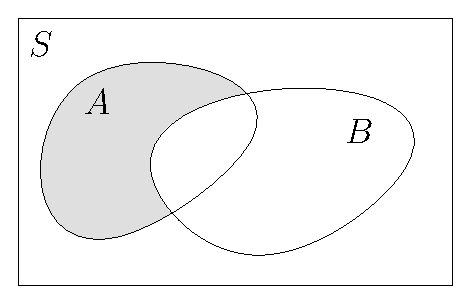
\includegraphics[height=20mm]{diagram4.eps}
%$\overline A$:
%
\includegraphics[height=20mm]{diagram5.eps}
%
%\medskip
%Of course such ``drawing'' has no connection with proposition proving.

\section{Power set}

The {\em power set} of a given set $A$ is the family of sets that contains as elements
precisely all the subsets of the set $A$:
$${\cal P}(A) = \{X; X\subseteq A\}$$

\textbf{ Example:}
\begin{itemize}
  \item ${\cal P}(\{1,2\}) = \{\emptyset, \{1\},\{2\},\{1,2\}\}$
  \item ${\cal P}(\emptyset) = \{\emptyset\}$.
  \item ${\cal P}(\{\emptyset\}) = \{\emptyset, \{\emptyset\}\}$.
\end{itemize}

If a set $A$ has $n$ elements, then its power set ${\cal P}(A)$ has  $2^n$ elementov.\footnote{For each of the $n$ elements of $A$ we need to decide, independently of the other elements, whether to include it in $X\subseteq A$ or not. Thus, altogether we have $n$
independent choices of one out of two possibilities, which, for all subsets $X\subseteq A$, gives us exactly $2^n$ possobilities.}

\bigskip
Properties:
\begin{itemize}
  \item $A\subseteq B\sledi \P(A) \subseteq \P(B)$.
  \item $\P(A) \cup \P(B) \subseteq \P(A\cup B)$.
  \item $\P(A)\cap \P(B) =  \P(A\cap B)$.
\end{itemize}

The first property follows from transitivity of inclusion:

$X\in \P(A) \inn A\subseteq B\cee X\subseteq A\subseteq B\sledi X\subseteq B\cee X\in \P(B)$.

Proof of the second property:

$X\in \P(A) \cup \P(B) \cee X\subseteq A\ali X\subseteq B\sledi X\subseteq A\cup B\cee X\in \P(A\cup B)$.

Proof of the third property:

$X\in \P(A)\cap \P(B)\cee X\in \P(A) \inn A\in \P(B)\cee X\subseteq A \inn X\subseteq B$

$\cee X\subseteq A \cap B\cee X\in \P(A\cap B)$

%\textbf{ V razmislek:} Zakaj velja predzadnja equivalence v zgornji verigi ekvivalenc?
%
%\medskip
%\textbf{ Homework:} Formalno dokažite prvo and drugo lastnost.

\textbf{ A question:} Why in the second property we don't have equality?


%\newpage
% 10. predavanje: 15.11.2011, malo manj kot 2 uri

\bigskip

%1. Dokažimo ekvivalenco
%$$A\subseteq B\cee A\cap B = A\,.$$
%
%\medskip
%$(\Leftarrow)$: $A=A\cap B\subseteq B$.
%
%\medskip
%$(\Rightarrow)$:
%Let $A\subseteq B$.
%
%Pokazati moramo: $(A\cap B\subseteq A)\inn(A\subseteq A\cap B)$.
%
%$A\cap B\subseteq A$ vselej velja.
%
%Dokažimo relacijo $A\subseteq A\cap B$ s contradictionm.
%
%Recimo, da
%$(\exists x)(x\in A\inn x\not\in A\cap B)$.
%
%$\sledi (\exists x)(x\in A\inn \neg(x\in A \inn x\in B))$
%
%$\sledi (\exists x)(x\in A\inn (x\not\in A \ali x\not \in B))$
%
%$\sledi (\exists x)((x\in A\inn x\not\in A) \ali (x\in A\inn x\not \in B))$
%
%$\sledi (\exists x)(x\in A\inn x\not \in B)$
%
%$\sledi \neg (\forall x)(x\in A\sledi x\in B)$
%
%To pa je contradiction s predpostavko $A\subseteq B$.
%
%\bigskip

\textbf{ Solution of one of the homeworks:}

Let us show that for every three subsets $A$, $B$, $C$, it holds that:
$$(A\cap B)\cup C = A\cap (B\cup C) \cee C\subseteq A\,.$$

\medskip
$(\Rightarrow)$:
Suppose that $(A\cap B)\cup C = A\cap (B\cup C)$.

$C\subseteq (A\cap B)\cup C = A\cap (B\cup C)\subseteq A$. We use transitivity of inclusion.

\medskip
$(\Leftarrow)$:
Suppose that $C\subseteq A$. Then $A\cup C = A$.

Consequently
$(A\cap B)\cup C = (A\cup C)\cap (B\cup C) = A\cap (B\cup C)$.\kz


\bigskip

Let us prove one of De Morgan's laws for an arbitrary set family
${\cal A} = \{A_\lambda~;~\lambda\in J\}$:

$$\overline{\cup_{\lambda\in J}A_\lambda} = {\cap_{\lambda\in J}\overline A_\lambda}$$
\begin{align*}
    x\in \overline{\cup_{\lambda\in J}A_\lambda}
& \cee
x\not\in \cup_{\lambda\in J}A_\lambda
\cee
\neg(\exists \lambda)(\lambda \in J\inn x\in A_\lambda)
\cee 
\\
&\cee(\forall \lambda)(\lambda \in J\sledi \neg(x\in A_\lambda))
\cee \\
& \cee
(\forall \lambda)(\lambda \in J\sledi x\in \overline{A_\lambda})
\cee
x\in {\cap_{\lambda\in J}\overline A_\lambda}\,.
\end{align*}

\section{Ordered pairs and tuples}

Consider two objects $a$ and $b$, $a\neq b$.
For the set $\{a,b\}$ the order is irrelevant, $\{a,b\} = \{b,a\}$.
When the order of elements is important, we speak about an {\em ordered pairs}:

$(a,b)$ - ordered pair, $(a,b)\neq (b,a)$
\begin{itemize}
    \item $a$ - first coordinate
    \item $b$ - second coordinate
\end{itemize}
When are two ordered pairs the same?
$$(a,b) = (u,v) \cee a = u \inn b = v\,.$$

\medskip
\textbf{ Remark:}
Ordered pairs $(a,b)$ or ordered structures of length $k$ (called ordered $k$-tupkes can also be defined as follows.
\medskip

\textbf{Definition:} 
The ordered $k$-tuple is an ordered sequence of elements denoted by normal brackets, i.e. $(a_1,a_2,\dots,a_k)$.
Formally we may encode the ordered $k$-tuple $(a_1,a_2,\dots,a_k)$ as an ordinary set
\[
(a_1,a_2,\dots,a_k)=\{A_1,A_2,\dots,A_k\},
\]
where $A_i={a_i,a_{i+1},\dots,a_k}$ for any $1\le i\le k$. 
Usually we use only ordered $2$-tuples, which are also called ordered pairs.

\medskip
\textbf{ Homework:}
Prove that $$\{\{a\},\{a,b\}\} = \{\{u\},\{u,v\}\}\cee a = u \inn b = v\,.$$

\section{Cartesian product}

The {\em Cartesian product} of sets $A$ and $B$ is the set that contains as elements precisely all the ordered pairs $(x,y)$ such that
 the first coordinate is from $A$ and the second coordinate is from $B$:
 $$A\times B = \{(x,y)~;~x\in A\inn y\in B\}$$

\textbf{ Example:} $\{1\}\times \{2,3\} = \{(1,2),(1,3)\}$,

$\{2,3\}\times \{1\} = \{(2,1),(3,1)\}$.

\bigskip
Properties of the Cartesian product:
\begin{itemize}
  \item $A\times B\neq B\times A$ (unless $A = B$)
  \item $A\times B = \emptyset \cee A= \emptyset \ali B = \emptyset$.
  \item $A\times (B\cup C) = (A\times B) \cup (A\times C)$.
  \item $A\times (B\cap C) = (A\times B) \cap (A\times C)$.
  \item $A\times (B\brez C) = (A\times B) \brez (A\times C)$.
\end{itemize}

The Cartesian product of three sets can be defined as:

$$A\times B\times C = (A\times B)\times C= \{((x,y),z)~;~x\in A \inn y\in B\inn z\in C\}\,.$$

Usually, we write just: $((x,y),z) = (x,y,z)$ (ordered triple).

\bigskip
The Cartesian product of sets $A_1,\ldots, A_n$ is defined as the set of all ordered
$n$-tuples:
$$A_1\times A_2\times\cdots \times A_n = \prod_{i = 1}^n A_i = \{(x_1,\ldots, x_n)~;~x_1\in A_1\inn x_2\in A_2\inn\cdots \inn x_n\in A_n\}\,.$$


\section*{A short discussion about axioms}

Every mathematical theory is based on a set of axioms --- basic propositions that we {\ em assume} to be correct.
These axioms define the basic properties that objects of a certain theory should satisfy (e.g.~integers, real numbers, groups, vector spaces, graphs, manifolds, ...). From the axioms new truths (claims, consequences, theorems ...) are derived by logical reasoning.

In Set Theory, the situation is the same! There are several families of axioms, but the most established are seven particular axioms, called {\em axioms of ZFC} (Zermelo - Fraenkel - (Axiom of) Choice), see Appendix.

These axioms ensure the existence of sets and ways of forming new sets from existing ones. 
Except for the Axiom of Choice, which is of special interest, we will not discuss other axioms here in detail.

\chapter{Relations}

Within every mathematical theory ${\cal T}$ with universal set $S$
we can represent every meaningful property $P(x)$
with the set $$\{x~;~x\in S\inn P(x)\}\,.$$
Similarly, we can also represent {\em relations} with sets.

\medskip
Examples of binary relations: $\in$, $\subseteq$, $=$, $\le$, $>$, parallel, congruent
\begin{itemize}
          \item Example: 3 and 5 are in relation ``smaller".
\end{itemize}
Ternary relations: sum, difference, product

------

``Family'' relations: father, son, mother, husband, mother-in-law, $\ldots$

parents -- ternary relation ($x,y,z$ are in the relation if and only if $x$ and $y$ are parents of $z$)

------
\section{Basic notions for binary relations}

Let $R$ be a meaningful binary relation for some mathematical theory ${\cal T}$ with universal set $S$.

$R$ will be presented with the set of exactly those ordered pairs of elements of $S$
whose first coordinate is in relation $R$ with the second coordinate.

$x$ is in relation $R$ with  $y$: $xRy$ or $R(x,y)$.
$$R = \{(x,y)~;~x,y\in S\inn xRy\}$$
or simply (if the universal set $S$ is clear from the context):
$$R = \{(x,y)~;~xRy\}\,.$$

\medskip
If $R$ is $n$-ary, we use $n$-tuples:
$$R = \{(x_1,\ldots, x_n)~;~R(x_1,\ldots, x_n)\}$$

------

A binary relation is therefore \textbf{ a subset of the Cartesian product} $S \times S =: S^2$.

An $n$-ary relation is a subset of the $n$-fold Cartesian product of set $S$ with itself,
$S \times \cdots \times S = \Pi_ {i = 1}^nS =: S^n$.

\bigskip
\zgled

$S = \{1,2,3,4\}$,

Binary relation ``smaller'', $<(x,y) \cee x<y$:

$$< = \{(1,2),(1,3),(1,4), (2,3), (2,4), (3,4)\}\,.$$

Ternary relation ``sum'', $+(x,y,z) \cee x+y = z$:

$$+ = \{(1,1,2),(1,2,3),(1,3,4), (2,1,3), (2,2,4), (3,1,4)\}\,.$$
\kz

\bigskip

\zgled

$S = \{1,2,3,4,5,6\}$,

Binary relation $R$ ``multiple'', $R(x,y) \cee x$ is a multiple of $y$, that is,

$(\exists k)(k$ is a positive integer and $x = k\cdot y$):
$$R = \{(1,1),(2,1),(2,2),(3,1),(3,3),(4,1),(4,2),(4,4),(5,1),(5,5),(6,1),(6,2),(6,3),(6,6)\}\,.$$

Ternary relation ``product'', $\cdot(x,y,z) \cee z = x\cdot y$:
$$\cdot  = \{(1,1,1),(1,2,2),(1,3,3),(1,4,4),(1,5,5),(1,6,6),(2,1,2),$$$$(2,2,4),(2,3,6),(3,1,3),(3,2,6),(4,1,4),(5,1,5),(6,1,6)\}\,.$$

``Unary'' relation ``prime'', $P(x) \cee x$ is a prime:

$P = \{2,3,5\}$.
\kz

\bigskip

Since we represented relations with sets, we can also speak about relations
$R\cup T$, $R\cap T$, $R\brez T$.

\bigskip
\zgled
Let us denote by $R_{\leq}$, $R_{<}$, $R_{=}$, $R_{\ge}$, $R_{>}$ and $R_{\neq}$
respectively the relations ``smaller or equal'', ``smaller'', ``equal'',
``greater or equal'', ``greater'' and ``non-equal'' (e.g., on the set of positive integers). Then:
%$$(x\leq  y) = (x<y) \cup (x = y)$$
%$$(x> y) = (x\ge y) \brez (x = y)$$
%$$(x> y) = (x\ge y) \cap (x \neq y)$$
$$R_\leq = R_< \cup R_=$$
$$R_> = R_\ge \brez R_= = R_\ge \cap R_{\neq}$$
\kz

\bigskip

Let us now focus on \textbf{ binary relations} (these are of particular interest, as we shall see in the chapter on order structures).

Let $R$ be a binary relation on a universal set $S$:
$$R = \{(x,y)~;~xRy\}\,.$$

The set of all first coordinates of elements of $R$ is said to be the {\em domain of relation $R$.}

The set of all second coordinates of elements of $R$ is said to be the {\em range (codomain) of relation $R$.}

Domain: $${\cal D}R = \{x~;~(\exists y)(xRy)\}$$
Range: $${\cal R}R = \{y~;~(\exists x)(xRy)\}$$

\medskip

\zgled

$R = \{(1,2), (2,3), (2,4)\}$.

${\cal D}R = \{1,2\}$,

${\cal R}R = \{2,3,4\}$

\kz

\bigskip

------

\textbf{ Inverse relation:}
$$R^{-1}= \{(y,x)~;~xRy\}$$
Clearly:
\begin{itemize}
  \item $yR^{-1}x \cee xRy\,.$
  \item ${\cal D}R^{-1} = {\cal R}R$ and ${\cal R}R^{-1} = {\cal D}R$.
    \item $(R^{-1})^{-1} = R$.
\end{itemize}


\bigskip
\zgled

 $R_\le^{-1}~~=~~R_\ge\,,$

 $R_<^{-1}~~=~~R_>\,,$

 $R_=^{-1}~~=~~R_=\,,$

$R_{\neq}^{-1}~~=~~R_{\neq}\,.$\kz

\subsection{Composition of relations}

Let $R$ and $T$ be two binary relations.

$T\circ R$: composition of relation $R$ with relation $T$

$$x T\circ R y \cee (\exists u)(xRu\inn uTy)$$

$$T\circ R = \{(x,y)~;~(\exists u)(xRu\inn uTy)$$


\bigskip
\zgled

$R = \{(1,3),(2,3)\}$, $T = \{(3,1)\}$

$T\circ R = \{(1,1), (2,1)\}$, $R\circ T = \{(3,3)\}$.


\medskip

brother $\circ$ father $\subseteq$ father

father $\circ$ brother  $\subseteq$ uncle

(father $\circ$ brother)$\cup$(mother $\circ$ brother) = uncle

sister $\circ$ mother $\subseteq$  mother

(wife $\circ$ mother) $\cup$ (husband $\circ$ mother) = mother-in-law
\kz

\medskip
In general $T\circ R\neq R\circ T$. On the other hand, associativity holds.

\begin{proposition}
Let $V, T, R$ be binary relations on universal set $S$. Then
$$V\circ(T\circ R) = (V\circ T)\circ R\,.$$
\end{proposition}

\begin{proof}
$$(x,y)\in V\circ(T\circ R)\cee x V\circ(T\circ R) y
\cee$$
$$(\exists u)(x(T\circ R)u\inn uVy)
\cee (\exists u)(\exists v)(xRv\inn vTu\inn uVy)\cee $$
$$(\exists v)(xRv\inn (\exists u)(vTu\inn uVy))
\cee(\exists v)(xRv\inn v(V\circ T)y)\cee$$
$$x ((V\circ T)\circ R)y \cee (x,y)\in (V\circ T)\circ R\,.$$
\end{proof}

Inverse of a  composition is equal to the composition of inverses in reverse order:

\begin{proposition}
Let $T$ and $R$ be binary relations on universal set $S$. Then
$$(T\circ R)^{-1} = R^{-1}\circ T^{-1}\,.$$
\end{proposition}

\begin{proof}
$$(x,y)\in (T\circ R)^{-1} \cee (y,x)\in T\circ R
\cee$$
$$(\exists u)(yRu\inn uTx)
\cee (\exists u)(uR^{-1}y\inn xT^{-1}u)
\cee$$
$$(\exists u)(xT^{-1}u\inn uR^{-1}y)
\cee x (R^{-1}\circ T^{-1}) y\cee (x,y)\in R^{-1}\circ T^{-1}\,.$$
\end{proof}


\bigskip
\zgled

Let  $a,b\in\mathbb{R}$.

Define the following relations

$R = \{(x,y)~;~x+y = a\}$,

$T = \{(x,y)~;~x+y = b\}$.

Then
$T\circ R = \{(x,y)~;~(\exists u)(x+u = a\inn u+y = b)\}=\{(x,y)~;~x-y = a-b\}$.

$R\circ T = \{(x,y)~;~x-y = b-a\}$.

$R^{-1}= R$, $T^{-1} = T$.

In this case, equality in the above claim becomes
$(T\circ R)^{-1} = R \circ T\,.$
\kz



\subsection{Universal, null and identity relations}

Every set $S$ asmits three special relations:

$S\times S$ -- the universal relation

$\emptyset$ -- the null relation

$I = \{(x,x)~;~x\in S\}$ -- the identity relation

\begin{proposition}
Let $R$ be a binary relation on universal set $S$.

Then $I\circ R = R\circ I = R$.
\end{proposition}

\begin{proof}
$xI\circ Ry \cee (\exists u)(xRu \inn uIy) \cee xRy$.

$xR\circ Iy \cee (\exists u)(xIu \inn uRy) \cee xRy$.
\end{proof}

\medskip
It also holds:

\begin{itemize}
  \item $\emptyset \circ R = R\circ \emptyset = \emptyset$
  \item $(S\times S)\circ R =
({\cal D}R) \times S$ and $R\circ (S\times S) = S\times {\cal R}R$.
\end{itemize}

%Let us prove the equality $R\circ (S\times S) = S\times {\cal R}R$:
%
%$x(R\circ (S\times S))y \cee (\exists u)(x(S\times S)u \inn uRy)
%\cee (\exists u)(uRy) \cee y\in {\cal R}R \cee x\in S\inn y\in {\cal R}R  \cee x(S\times {\cal R}R)y$.

\bigskip

\textbf{ Homework}: Prove the above properties.
%equality $(S\times S)\circ R = ({\cal D}R) \times S$.

%$x((S\times S)\circ R)y \cee (\exists u)(x R u \inn u(S\times S)y)
%\cee (\exists u)(xRu) \cee x\in {\cal D}R \cee x\in {\cal D}R\inn y\in S  \cee x(({\cal D}R) \times S)y$.

\section{Properties of binary relations}

Some properties of binary relations are particularly important:

\bigskip

$R \textrm{ is {\em reflexive}} \cee (\forall x)(x\in S\sledi xRx)$

%\begin{center}
%\includegraphics[height=20mm]{reflexive.eps}
%\end{center}

\textbf{ Example:} relation $\le$ in real numbers

\bigskip

$R \textrm{ is {\em irreflexive}} \cee (\forall x)(x\in S\sledi \neg(xRx))$

%\begin{center}
%\includegraphics[height=20mm]{irreflexive.eps}
%\end{center}

\textbf{ Example:} relation  $<$ in real numbers

\bigskip

$R \textrm{ is {\em symmetric}} \cee (\forall x)(\forall y)(x\in S\inn y\in S\inn xRy\sledi yRx)$

%\begin{center}
%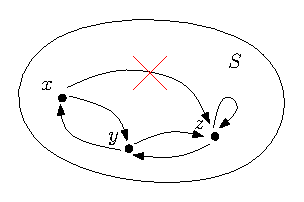
\includegraphics[height=20mm]{simetricna.eps}
%\end{center}
%

\textbf{ Example:} relation ``being parallel'' on lines in the plane

\bigskip

$R \textrm{ is {\em asymmetric}} \cee (\forall x)(\forall y)(x\in S\inn y\in S\inn xRy\sledi \neg(yRx))$

%\begin{center}
%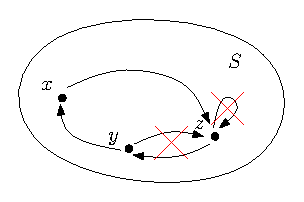
\includegraphics[height=20mm]{asimetricna.eps}
%\end{center}

\textbf{ Example:} relation  $<$ in real numbers

% 12. predavanje, 2 uri, 22. 11. 2011

%Pokazali smo, da velja ${\cal P}(A)\cup {\cal P}(B)\subseteq  {\cal P}(A\cup B)$.
%
%Dokaži, da velja
%$${\cal P}(A)\cup {\cal P}(B)={\cal P}(A\cup B)$$
%natanko tedaj, ko je $$(A\subseteq B) \ali (B\subseteq A)\,.$$.
%
%\bigskip
%${\cal P}(A)\cup {\cal P}(B)={\cal P}(A\cup B)$
%
%$\cee$
%
%${\cal P}(A\cup B) \subseteq {\cal P}(A)\cup {\cal P}(B)$
%
%$\cee$
%
%$(\forall X)(X\in {\cal P}(A\cup B)\sledi X\in {\cal P}(A)\cup {\cal P}(B))$
%
%$\cee$
%
%$(\forall X)(X\subseteq A\cup B\sledi X\subseteq A \ali X\subseteq B)$
%
%$\cee$
%
%$(A\subseteq B) \ali (B\subseteq A)$
%
%\medskip
%Dokaz zadnje ekvivalence napravimo posebej:
%
%$(\Leftarrow)$:
%Èe je $(A\subseteq B) \ali (B\subseteq A)$, potem je
%$A\cup B = B \ali A\cup B = A$ and v vsakem primeru velja
%$(\forall X)(X\subseteq A\cup B\sledi X\subseteq A \ali X\subseteq B)$.
%
%\medskip
%
%$(\Rightarrow)$:
%Recimo, da je
%$(\forall X)(X\subseteq A\cup B\sledi X\subseteq A \ali X\subseteq B)$
%and da ne velja
%$(A\subseteq B) \ali (B\subseteq A)$.
%
%Torej je
%$\neg((A\subseteq B) \ali (B\subseteq A))$
%
%$\sledi$
%
%$(\neg(A\subseteq B) \in \neg(B\subseteq A))$
%
%$\sledi$
%
%$(\exists a)(a\in A\brez B)\inn (\exists b)(b\in B\brez A)$.
%
%Tedaj pa za množico $X = \{a,b\}$ velja $X\subseteq A\cup B$, vendar ne velja $X\subseteq A$ niti $X\subseteq B$.
%contradiction.\hfill\qed
%
%\bigskip
%
%\textbf{ Ponovitev:}
%
%binarne relacije
%
%domena
%
%zaloga vrednosti
%
% \zgled
%
%Let $X$ poljubna set and $S = X\cup {\cal P}(X)$. relation  $R$ je podmnožica $S\times S$, definirana s predpisom
%$$xRy\cee x\in X\inn x\in y\,.$$
%Tedaj je ${\cal D}R = X$ and ${\cal R}R = {\cal P}(X)\brez \{\emptyset\}\,.$
%\kz
%
%\medskip
%Inverzna relation . Kompozitum relacij.
%
%$x(T\circ R)y \cee (\exists u)(xRu\inn uTy)$.
%
%$(R\circ T)^{-1} = T^{-1}\circ R^{-1}$
%
%nièelna relation , identièna relation ,
%univerzalna relation
%
%\bigskip
%
%Rešitev domaèe  naloge:  $(S\times S)\circ R = ({\cal D}R) \times S$.
%
%\bigskip
%
%$R \textrm{ is {\em reflexive}} \cee (\forall x)(x\in S\sledi xRx)$
%
%$R \textrm{ is {\em irreflexive}} \cee (\forall x)(x\in S\sledi \neg(xRx))$
%
%$R \textrm{ is {\em symmetric}} \cee (\forall x)(\forall y)(x\in S\inn y\in S\inn xRy\sledi yRx)$
%
%$R \textrm{ is {\em asymmetric}} \cee (\forall x)(\forall y)(x\in S\inn y\in S\inn xRy\sledi \neg(yRx))$
%
%\bigskip

\bigskip

$R \textrm{ is {\em antisymmetric}} \cee (\forall x)(\forall y)(x\in S\inn y\in S\inn xRy\inn yRx\sledi x = y)$
%
%\begin{center}
%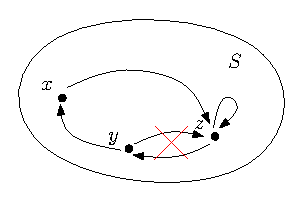
\includegraphics[height=20mm]{antisimetricna.eps}
%\end{center}

\textbf{ Example:}
relation  $\le$ in real numbers

relation  $\subseteq$ in sets

\bigskip

$R \textrm{ is {\em transitive}} \cee (\forall x)(\forall y)(\forall z)(x\in S\inn y\in S\inn z\in S\inn xRy\inn yRz\sledi xRz)$

%\begin{center}
%\includegraphics[height=20mm]{transitive.eps}
%\end{center}

\textbf{ Example:} relation  $<$ in real numbers

relation  $\subset$ in sets

\bigskip

$R \textrm{ is {\em intransitive}} \cee (\forall x)(\forall y)(\forall z)(x\in S\inn y\in S\inn z\in S\inn xRy\inn yRz\sledi \neg(xRz))$

%\begin{center}
%\includegraphics[height=20mm]{intransitive.eps}
%\end{center}

\textbf{ Example:}
relation  $R$ in real numbers, defined by the rule $xRy \cee x = y + 1$

\bigskip

$R \textrm{ is {\em strict total}} \cee (\forall x)(\forall y)(x\in S\inn y\in S
\inn x\neq y\sledi (xRy)\ali (yRx))$

%\begin{center}
%
\includegraphics[height=20mm]{sovisna.eps}
%\end{center}

\textbf{ Example:}
relation  $<$ in real numbers

\bigskip

$R \textrm{ is {\em total}} \cee (\forall x)(\forall y)(x\in S\inn y\in S
\sledi (xRy)\ali (yRx))$

%\begin{center}
%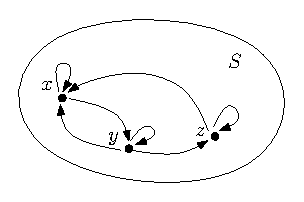
\includegraphics[height=20mm]{strogosovisna.eps}
%\end{center}

\textbf{ Example:}

relation  $\le$ in real numbers

\bigskip
\textbf{ Homework:}
Choose some family relations and for each of them verify which of the above properties hold.

\bigskip
Some of the above properties imply others:
\begin{itemize}
  \item $R$ is total $\sledi$ $R$ is strict total.
  \item $R$ is asymmetric $\sledi$ $R$ is irreflexive.
  \item $R$ is symmetric and transitive, and ${\cal D}R = S$ $\sledi$ $R$ is reflexive
\end{itemize}

% 13. predavanje, 2 uri, 23. 11. 2011

% 3. kviz


\section{Equivalence relation}

$R$ is {\em equivalence} $\cee$ $R$ is reflexive, symmetric and transitive.

\textbf{ Example:} the identity relation

\begin{proposition}
$R$ is equivalence $\cee$ ${\cal D}R = S$ and $R^{-1}\circ R = R$.
\end{proposition}

\begin{proof}
The condition is necessary:

$xRx \sledi {\cal D}R = S$
$$xR^{-1}\circ Ry \sledi (\exists z)(xRz \inn zR^{-1}y)
\sledi (\exists z)(xRz \inn yRz)
\sledi (\exists z)(xRz \inn zRy)
\sledi xRy\,.$$
$$xRy
\sledi (xRy\inn yRy)
\sledi (xRy\inn yR^{-1}y)
\sledi xR^{-1}\circ Ry\,.$$
Hence $R^{-1}\circ R = R$.

The condition is also sufficient:

Let ${\cal D}R = S$ and $R^{-1}\circ R = R$.

Reflexivity: we need to show  $(\forall x)(x\in S\sledi xRx)$.

Let $x\in S$. Since ${\cal D}R = S$,
it follows $x\in {\cal D}R\sledi (\exists y)(y\in S\inn xRy)$.
$$xRy
\sledi xRy\inn yR^{-1}x
\sledi x R^{-1}\circ R x
\sledi xRx\,.$$

Symmetry: we need to show $(\forall x)(\forall y)(x\in S\inn y\in S\inn xRy\sledi yRx)\,.$

Let $x\in S\inn y\in S\inn xRy$.
Then
$$xRy \sledi (xRy\inn yRy)
\sledi (yRy\inn yR^{-1}x)
\sledi yR^{-1}\circ Rx
\sledi yRx\,.$$

Transitivity: we need to show $(\forall x)(\forall y)(\forall z)(x\in S\inn y\in S\inn z\in S\inn xRy\inn yRz\sledi xRz).$

Let $x\in S\inn y\in S\inn z\in S\inn xRy\inn yRz$.
Then $$xRy \inn yRz \sledi xRy\inn zRy
\sledi xRy\inn yR^{-1}z
\sledi xR^{-1}\circ Rz
\sledi xRz\,.$$
\end{proof}

Every equivalence relation has the nice property that it divides set $S$ on which it is defined into {\em non-empty and pairwise disjoint sets the union of which is exactly set $S$}.

\medskip
\textbf{ Equivalence classes.}

Let $R$ be an equivalence relation defined on a set $S$. Let $x\in S$. The {\em equivalence class of element $x$ with respect to the equivalence relation $R$} is the set of all elements that are in relation with $x$:
$$R[x] = \{y~;y\in S \inn yRx\}\,.$$

Equivalence classes enjoy the following properties:
\begin{itemize}
  \item Since $R$ is a reflexive relation, it holds $x\in R[x]$. Consequently $R[x]\neq \emptyset$.
  \item $y\in R[x]\sledi R[y]=R[x]$.

  Indeed: Let $y\in R[x]$.

  $z\in R[y]\sledi zRy\inn yRx\sledi zRx\sledi z\in R[x]$.

  $z\in R[x]\sledi zRx\inn yRx\sledi zRx\inn xRy \sledi zRy\sledi z\in R[y]$.
  \item $y\not\in R[x]\sledi R[x]\cap R[y]=\emptyset$.

  Indeed: $(\exists z)(z\in R[x]\cap R[y])\sledi (\exists z)(R[z] = R[x]\inn R[z] = R[y])\sledi
  y\in R[y]=R[x]$. Contradiction with assumption $y\not\in R[x]$.
  \end{itemize}

It follows that:
\begin{enumerate}
  \item Every element of $S$ is in exactly one equivalence class. Namely in the one containing all elements of $S$ that are in relation $R$ with it.
  \item Every equivalence class is completely determined with an arbitrary element of it. We say that an arbitrary element of a class is a {\em representative} of the class.
      \item The equivalence classes of a given equivalence relation $R$ divide the set $S$ into
      nonempty and pairwise disjoint sets the union of which is the set $S$.
      \end{enumerate}

\begin{figure}[htp]
\begin{center}
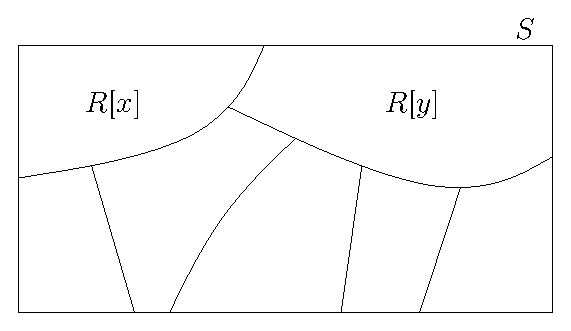
\includegraphics[height=30mm]{ekvivalencna.eps}
\end{center}
\end{figure}

Such divisions are called partitions. {\em Partition of a set $S$} = a set of nonempty and pairwise disjoint sets the union of which is $S$.

Hence, to every equivalence relation there corresponds a partition of set $S$.
The converse holds as well. Every partition ${\cal A}$ of set $S$ determines a unique equivalence relation $R$
such that the sets in the partition are exactly the equivalence classes of relation $R$.
\begin{itemize}
  \item Two elements $x$ and $y$ are in relation $R$ if and only if they belong to the same set of the partition:
      $$xRy\cee (\exists X)(X\in {\cal A}\inn x\in X\inn y\in X)\,.$$
\end{itemize}
Let us verify that the so defined relation is an equivalence relation:
\begin{itemize}
  \item reflexivity: $x\in S \sledi (\exists X)(X\in {\cal A}\inn x\in X)\sledi xRx\,.$
  \item symmetry:
  $xRy\sledi (\exists X)(X\in {\cal A}\inn x\in X\inn y\in X)
  \sledi (\exists X)(X\in {\cal A}\inn y\in X\inn x\in X)\sledi yRx\,.$
  \item transitivity:
  $xRy \inn yRz\sledi (\exists X)(X\in {\cal A}\inn x\in X\inn y\in X)
  \inn (\exists Y)(Y\in {\cal A}\inn y\in Y\inn z\in Y)$.

  Hence $y$ is both in $X$ and $Y$. Since the sets are pairwise disjoint, it follows that
  $X = Y$. But then $z$ is also in set $X$. Consequently $xRz$.
\end{itemize}

\textbf{ Exercise:} Justify that partition ${\cal A}$ coincides with the set of equivalence classes of relation $R$.

\bigskip

% 14. predavanje, 2 uri, 29. 11. 2011

To every set $S$ on which some equivalence relation $R$ is defined, we can associate some new set, the elements of which are the equivalence classes of relation $R$:

{\em Quotient set of $S$ with respect to relation $R$}:
$$S/R = \{R[x]~;~x\in S\}=\{X~;~(\exists x)(x\in S \inn X = R[x])\}$$
\begin{itemize}
  \item The notion of quotient set represents a mathematical formulation of the logical notion of {\em abstraction}:
  By moving from a given set $S$ to the quotient set, we ignore all differences between objects belonging to the same equivalence class!
\end{itemize}


\bigskip
\zgled

Let $S = \{1,2,3\}$ and $R = \{(1,1),(1,3),(2,2),(3,1),(3,3)\}$.

Relation  $R$ is an equivalence relation.

$R[1] = R[3] = \{1,3\}$, $R[2] = \{2\}$.

$S/R =  \{R[1], R[2],R[3]\} = \{R[1], R[2]\} = \{\{1,3\},\{2\}\}$.

If we define a partition ${\cal A} = \{\{1,2\},\{3\}\}$ of set $S$, then we can define a relation $R'$ by the rule
$xR'y \cee (\exists X)(X\in {\cal A}\inn x\in X\inn y\in Y)$.
It holds

$R' = \{(1,1),(1,2),(2,1),(2,2),(3,3)\} = R$
and $S/R' = \{\{1,2\},\{3\}\} = {\cal A}$.
\kz


\subsubsection{Examples of equivalence relations}

\begin{enumerate}
\item \textbf{ Fractions.}

In the set of fractions $a/b\,,$
   where $ a $ and $ b $ be arbitrary integers and $ b \neq 0$, the definition of equality of two fractions
   $a / b = c / d \cee ad = bc$
    is an equivalence relation. Each equivalence class with respect to this relation collects together all pairwise equal fractions and then represents the corresponding {\em rational number}. The corresponding quotient set is the {\em set of rational numbers}.
   \item \textbf{ Congruences.}


   In the set of {\em integers} the relation {\em congruence modulo $m$}, where $ m> 0$  is a positive integer, $$a \equiv b \pmod{m} \cee m \textrm{ divides } a-b \,,$$
   is an equivalence relation.

   In this case, the equivalence classes are the {\em residue classes modulo $ m $}. Each equivalence class contains all those numbers that give the same remainder (residue) when divided by $ m $.

   Obviously there are exactly $ m $ of these classes. These classes are called {\em integers modulo $ m $}. The quotient set is the set of integers modulo $m$.

   \item \textbf{ Parallelism of lines.}

In the set of {\em all lines}, the relation ``parallel'' is an equivalence relation. Each equivalence class therefore contains all the lines that are parallel to each other, and therefore represent a certain {\em direction}. In this case, the quotient set is {\em the set of all directions}.
\end{enumerate}

\section{Functions}

{\em Function is a central notion of classical and modern mathematics.
From $18$th century on, the notion of a function was becoming increasingly
more precise and general. The definition of a function as we know it today was given by Cauchy and Riemann:}

\medskip
%Znana je naslednja definicija:
For two sets $A$ and $B$, a {\em function from $A$ to $B$} is a rule that assigns to every element of $A$ a unique element of $B$.
Notation: $f:A\to B$.

\medskip
To avoid any doubt what is meant with the word ``rule'', we can define functions as special relations.

\medskip
A binary relation $R$ is {\em unique} if:
$$(x,y)\in R \inn (x,z)\in R\sledi y = z$$

A {\em function} (also {\em mapping, map, transformation})
is a unique binary relation. We usually denote functions with letters $f, g,h,\ldots$

We say that $f$ is a function from $A$ to $B$, and write $f:A\to B$ if ${\cal D}f= A$ and the following holds: $(x,y)\in f\sledi x\in A\inn y\in B$.

The set of all functions from $A$ to $B$ is denoted by $B^A$.

We write
$$y=f(x)\cee (x,y)\in f\,.$$
$$f = \{(x,y)~;~x\in A\inn y = f(x)\in B\}\,.$$

$x\in A$: independent variable, original, argument

$y (= f(x))$: dependent variable, image of element $x$.

\medskip

The following notation is also in use:

$x\mapsto f(x)$~~``$x$ maps to  $f(x)$",

$A\overset{f}{\to} B$~~``$f$ is a function from $A$ to $B$".

\bigskip
\textbf{ Examples of functions:}
\begin{itemize}
  \item $A = \{1,2,3\}$, $B = \{2,4,6\}$

  $f = \{(1,2),(2,4),(3,4)\}$

  \item $A = \{$points at the surface of planet Earth$\}$, $B = \mathbb{R}$,

$f(x) = $ temperature in  $^\circ C$ at point $x$ on December 2, 2012, at 6:00 local time

  \item $A = \{$people living on Earth at a certain time $T\}$, $B = \mathbb{N}$,

$f(x) = $ age (in seconds) of person $x$ at time $T$.
\end{itemize}

\bigskip
The set $\{(x,y)~;~x\in A\inn y = f(x)\}$ is sometimes referred to as the {\em graph of a function.}

\bigskip
\textbf{ Depictions of functions.}
If $A\subseteq \mathbb{R}$ and $B = \mathbb{R}$, the graph of a function can also be depicted as
a set of points in the plane.

\textbf{ Example:} $f:\mathbb{R}\to \mathbb{R},~~~f(x) = x^2\,.$
\begin{center}
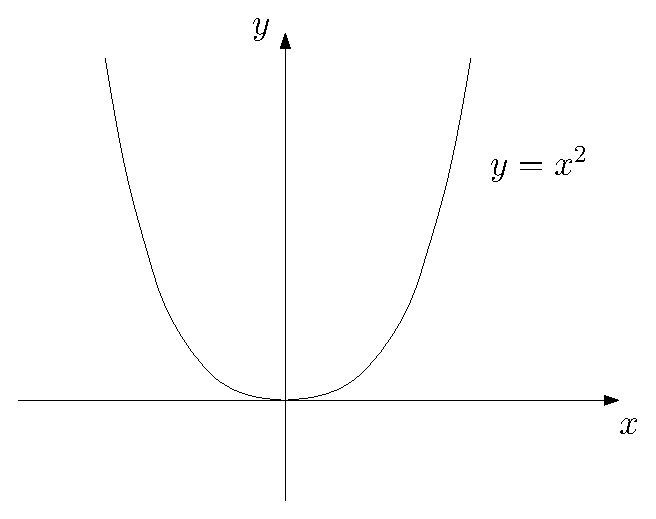
\includegraphics[height=50mm]{yx2.eps}
\end{center}

\medskip

In a asimilar way, we can also depict {\em binary relations} on the set $S =\mathbb{R}$:

Let $xRy \cee x^2+y^2 = 4$.
Then, relation $R$ is represented by a circle of radius $2$ and center in the origin.

\begin{center}
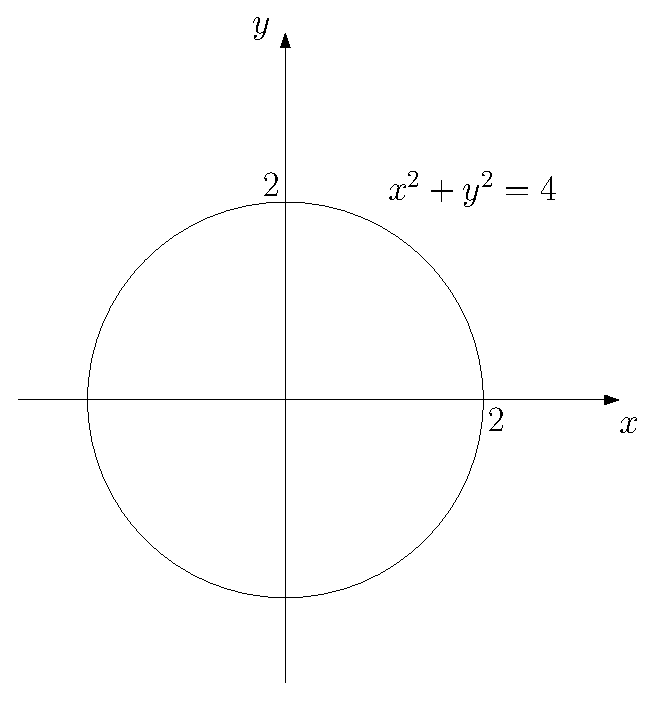
\includegraphics[height=50mm]{x2+y2=4.eps}
\end{center}

\bigskip
Let $f:A\to B$.
The domain of function $f$:

$${\cal D}f = \{x~,~(\exists y)((x,y)\in f)\} = A$$

Range of function $f$:

$$\textrm{Im}f = \{y~,~y\in B\inn (\exists x)(x\in A\inn (x,y)\in f)\} \subseteq B$$

%Množico vseh funkcij iz $A$ v $B$ lahko zapišemo s pomoèjo
%$$B^A = \{f~;~f\textrm{ is funkcija }\inn {\cal D}f = A \inn \textrm{ Im}f \subseteq B\}$$.

\medskip
\textbf{ Example:} $f = \{(1,2),(2,4),(3,4)\}$, $A = \{1,2,3\}$, $B = \{2,4,6\}$.
${\cal D}f = \{1,2,3\}$, $\textrm{Im}(f) = \{2,4\}$.

\bigskip
In general $\textrm{Im}f \subseteq B$. If equality holds, $\textrm{Im}f  = B$, then we say that $f$ is a {\em surjective} function.
In this case we say that $f$ maps $A$ {\em onto} $B$.

\bigskip
\textbf{ Example:} $A = \{1,2,3\}$, $B = \{2,4,6\}$. $f= \{(1,2),(2,4),(3,4)\}$ is not surjective. $g:A\to B$, $g = \{(1,2),(2,6),(3,4)\}$, is surjective.

\bigskip
The definition of a function allows that several originals have the same $f$-image.
In the extreme case, $f$ maps all elements of $A$ into the same element of $B$.
Such a function is called a {\em constant (function)}.

The other extreme occurs when two different originals always have different images:

$f$ is {\em injective} $\cee$ $(\forall y)(y\in \textrm{Im}f\sledi (\exists!x)(x\in A \inn f(x) = y))$

~~~~~~~~~~~~~~~$\cee$ $(\forall x)(\forall y)(f(x) = f(y) \sledi x = y)$

\bigskip
\textbf{ Example:} $f = \{(1,2),(2,4),(3,4)\}$ is not injective.
$g = \{(1,2),(2,6),(3,4)\}$ is injective.

\bigskip
Let $U\subseteq A$. We write:
$$f(U) = \{y~;~y\in B\inn (\exists x)(x\in U\inn f(x) = y)\}$$
$f(U)$ -- image of subset  $U$ under mapping $f$

\bigskip
\textbf{ Example:} $f = \{(1,2),(2,4),(3,4)\}$.
$U = \{2,3\}$. $f(U) = \{f(2),f(3)\} = \{4\}$.

\medskip
Clearly:
\begin{itemize}
  \item $f(A) = \textrm{Im}f$.
  \item $U\subseteq V\sledi f(U)\subseteq f(V)$.
\end{itemize}

The images behave in the following way with respect to unions and intersections:
\begin{itemize}
  \item $f(U\cup V) = f(U)\cup f(V)$,
  \item $f(U\cap V) \subseteq f(U)\cap f(V)$.
\end{itemize}

\textbf{ Homework:} Prove the above properties.

\subsection{Inverse relation, preimages}

\bigskip
\textbf{ Inverse relation:}
$$f^{-1} = \{(y,x)~;~f(x) = y\}\,.$$
$f^{-1}$ is not necessarily a function!

\medskip
\textbf{ Example:} $f = \{(1,2),(2,4),(3,4)\}$.
$f^{-1} = \{(2,1),(4,2),(4,3)\}$ - is not a function.

\medskip
{\em Preimage} of element $y$:
$$f^{-1}(y) = \{x~;~x\in A\inn f(x) = y\}\,.$$

Let $E\subseteq B$. {\em Preimage of $E$} (under mapping $f$):
$$f^{-1}(E) = \{x~;~x\in A\inn f(x) \in E\}$$

\medskip
\textbf{ Example:} $f = \{(1,2),(2,4),(3,4)\}$.
$f^{-1}(2) = \{1\}$, $f^{-1}(4) = \{2,3\}$, $f^{-1}(\{2,4\}) = \{1,2,3\}$
\medskip

Clearly:
\begin{itemize}
  \item $f^{-1}(\textrm{Im}f) = A$
\end{itemize}

\bigskip
It also holds:
\begin{itemize}
  \item $E\subseteq F\sledi f^{-1}(E)\subseteq f^{-1}(F)$
\end{itemize}

\bigskip
Preimages are in good relations with unions, intersections, and differences:
\begin{itemize}
  \item $f^{-1}(E\cup F)= f^{-1}(E)\cup f^{-1}(F)$
  \item $f^{-1}(E\cap F)= f^{-1}(E)\cap f^{-1}(F)$
  \item $f^{-1}(E\brez F)= f^{-1}(E)\brez f^{-1}(F)$
\end{itemize}

\textbf{ Proof of the property $f^{-1}(E\cap F)= f^{-1}(E)\cap f^{-1}(F)$:}
$$x\in f^{-1}(E\cap F)\cee
f(x)\in E\cap F\cee
f(x)\in E \inn f(x)\in F\cee$$ $$\cee x\in f^{-1}(E) \inn x\in f^{-1}(F)
\cee x\in f^{-1}(E)\cap f^{-1}(F)$$
\qed

\textbf{ Homework:} Prove the other two properties.

\bigskip
Similarly we can check that:
\begin{itemize}
  \item for all  $U\subseteq A$, it holds that $$U\subseteq f^{-1}(f(U))$$
  \item for all $E\subseteq B$, it holds that $$f(f^{-1}(E))\subseteq E$$
\end{itemize}

\bigskip

------------------------------------------------------------------------------------------------------------

\bigskip

Let $f:A\to B$. When is the inverse relation $f^{-1}$ a function?

$f^{-1}$ is a function from $\textrm{Im}f$ to  $A$ $\cee$ $f$ is injective.

%(Indeed: to have  da bo $f^{-1}$ funkcija, ne smeta obstajati dva razlièna urejena para v $f^{-1}$, ki bi imela isto prvo koordinato $\cee$ ne smeta obstajati dva razlièna urejena para v $f$, ki bi imela isto drugo koordinato, tj.~$f$ je injektivna.)


Therefore, if $f^{-1}$ is a function, then for every element
$y\in \textrm{Im}f$  there exists a unique $x\in {\cal D}f$ such that
$f^{-1}(y) = x$. It holds that
$$f^{-1}(y) = x\cee f(x) = y\,.$$

Hence: $$f^{-1}(f(x)) = x$$
and
$$f(f^{-1}(y)) = y\,.$$

A particularly interesting case is given if function $f$ is not only injective, but also surjective.
In this case, we say that function $f$ is {\em bijective}.

If $f$ is bijective, then  $\textrm{Im}f = B$ and $f^{-1}$ is a function from $B$ to $A$.

%\bigskip

%------------------------------------------------------------------------------------------------------------
%
%\bigskip

\subsection{Composition of functions}
$$g\circ f = \{(x,z)~;~(\exists y)((x,y)\in f\inn (y,z)\in g)\}$$
$$= \{(x,z)~;~(\exists y)(f(x) = y \inn g(y) = z)\}\,.$$

Hence, if $\textrm{Im}f\cap {\cal D}g = \emptyset$, then $g\circ f = \emptyset\,.$
This example is not particularly interesting, so we usually require: $\textrm{Im}f\subseteq {\cal D}g$,
therefore $A\overset{f}{\to} B\overset{g}{\to} C$.
Under this condition:
$$g\circ f = \{(x,z)~;~z = g(f(x))\}$$
relation $g\circ f$ is also a function (from $A$ to $C$): $(g\circ f)(x) = g(f(x))$.

\bigskip
\textbf{ Example:} $f = \{(1,2),(2,4),(3,4)\}$, $g = \{(2,3),(4,5)\}$
(Notice that ${\cal D}g = \textrm{Im}f$.)
$g\circ f = \{(1,3),(2,5), (3,5)\}$

\bigskip
Just like compositions of binary relations, compositions of functions also enjoy

\textbf{ Associativity:}

If
$$A\overset{f}{\to} B\overset{g}{\to} C\overset{h}{\to} D\,,$$
then
$$h\circ (g\circ f) = (h\circ g)\circ f\,.$$

\subsection{Restrictions and extensions}
When are two functions $f$ and $g$ the same?

According to the definition of equality of sets, $f = g$ only if they have the same ordered pairs as elements.
This is true precisely when the following two conditions are satisfied:
\begin{itemize}
  \item ${\cal D}f = {\cal D}g$
  \item for every element $x$ of this common domain, it holds $f(x) = g(x)$.
\end{itemize}

Two particular ways of modifying a given function are particularly important:

\textbf{ Restriction:}
Let $f:A\to B$ and $U\subseteq A$.

The {\em restriction} of $f$ on  $U$
is the function $g$ that has set $U$ as its domain and such that for all $x\in U$, it holds
$g(x) = f(x)$. Notation:
$$g = f_{|U}$$

\bigskip
\textbf{ Example:} $f = \{(1,2),(2,4),(3,4)\}$, $A = \{1,2,3\}$, $U =  \{1,2\}$.
$f_{|U} = \{(1,2),(2,4)\}$

\bigskip
If function $g$ is a restriction of function $f$, we say that $f$ is an {\em extension} of function $g$.

\subsection{Canonical decomposition of a function}
Consider the function $f:A{\to} B$.
Let us define the following relation $R$ on set $A$:
$$xRy \cee f(x) = f(y)\,.$$

Clearly, $R$ is an equivalence relation:
\begin{itemize}
  \item for all $x\in A$ it holds $xRx$,
  \item $xRy \sledi f(x) = f(y) \sledi f(y) = f(x) \sledi yRx$,
  \item $xRy \inn yRz \sledi f(x) = f(y) \inn f(y) = f(z) \sledi f(x) = f(z) \sledi xRz$.
\end{itemize}
Now, let us compute the quotient set $A/R$ (the set of all equivalence classes).

Let us first map set $A$ {\em onto} set $A/R$:
$$p:A{\to} A/R$$
$$p(a) = R[a]$$
Mapping $p$ is surjective. It is called a {\em natural mapping}.

Now, let us define a mapping $g$ from  the quotient set $A/R$ to set $B$ so that
function $f$ will be the composition of functions $p$ and $g$, $f = g\circ p$:
$$g:A/R{\to} B$$
$$g(u) = f(x)\,,$$
where $x$ is an arbitrary representative of equivalence class $u$ (that is, $x\in u$).

\begin{itemize}
  \item Mapping  $g$ is well defined (the value of $g(u)$ is independent of the choice of representative of class $u$):
$$x\in u\inn y\in u \sledi xRy \sledi f(x) = f(y)\,.$$
  \item Mapping $g$ is injective:
$$g(u) = g(v) \inn g(u) = f(x) \inn g(v) = f(y) \sledi f(x) = f(y) \sledi xRy \sledi  u = v\,.$$
  \item It follows from the definitions of functions $g$ and $p$ that  $f = g\circ p$:

Let $x\in A$. Then:
$$(g\circ p)(x) = g(p(x)) = g(R[x]) = f(x)\,.$$
\end{itemize}

We can decompose $f$ as follows:
\begin{center}
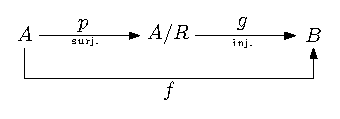
\includegraphics[height=20mm]{dekompozicija.eps}
\end{center}

%Izpeljali smo naslednjo dekompozicijo funkcije $f:A{\to} B$:
%\begin{center}
%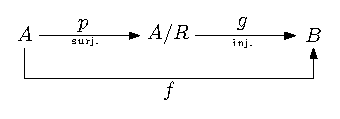
\includegraphics[height=20mm]{dekompozicija.eps}
%\end{center}
%
%Pri tem je:
%\begin{itemize}
%  \item  $p:A{\to} A/R$ surjektivna preslikava, definirana s predpisom
%$p(a) = R[a]$.
%  \item relation  $R$ je definirana na množici $A$ kot
%$xRy \cee f(x) = f(y)\,.$
%  \item $g:A/R{\to} B$ je injektivna preslikava, definirana s predpisom $g(u) = f(x)\,,$ kjer je $x\in u$.
%\item $f = g\circ p$.
%\end{itemize}
%
This decomposition can be further refined by
introducing a mapping $h$, given by the same rule as $g$, but that maps to the set $\textrm{Im}g = \textrm{Im}f$.
Mapping $h$ is then bijective:
$$h:A/R{\to} \textrm{Im}f$$
$$h(u) = g(u)\,.$$
Finally, we map set $\textrm{Im}f$ to set $B$ with the  {\em identity mapping} $i$, which fixes all elements:
$$i:\textrm{Im}f{\to}B$$
$$i(y) = y\,.$$

It is clear that for all $x\in A$, it holds
$$i(h(p(x))) = h(p(x)) = g(p(x)) = f(x)\,.$$
Therefore
$$f = i\circ h\circ p\,.$$
This way, we obtain {\em canonical decomposition} of function $f$:
\begin{center}
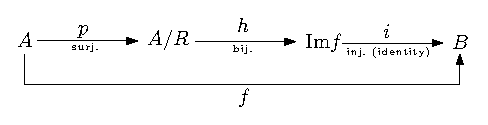
\includegraphics[height=20mm]{dekompozicija2en.eps}
\end{center}

\textbf{ Example:}
$A = \{1,2,3\}, B = \{2,4,6\}$,
$f = \{(1,2),(2,4),(3,4)\}$

(that is, $f(1) = 2$, $f(2)= f(3) = 4$)

Equivalence relation: $R = \{(1,1),(2,2),(3,3),(2,3),(3,2)\}$

Quotient set: $A/R = \{\{1\},\{2,3\}\}$

$\textrm{Im} f = \{2,4\}$

Natural mapping $p$: $p(1) = \{1\}$, $p(2) = p(3) = \{2,3\}$.

Mapping $g: \{\{1\},\{2,3\}\}\to \{2,4,6\}$:

$g(\{1\}) = f(1) = 2$, $g(\{2,3\}) = f(2) = f(3) = 4$.

Mapping $h: \{\{1\},\{2,3\}\}\to \{2,4\}$:
$h(\{1\}) = g(\{1\}) = 2$, $h(\{2,3\}) = g(\{2,3\}) = 4$.

Identity mapping $i:\{2,4\}\to\{2,4,6\}$: $i(2) = 2$, $i(4) = 4$.

\begin{center}
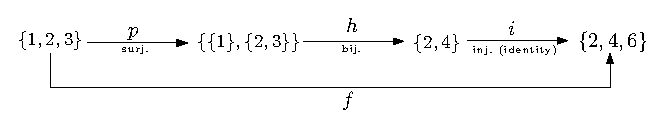
\includegraphics[height=20mm]{dekompozicija3en.eps}
\end{center}

%end of lectures 22.11
\newpage
\section{Order structures}

{\em Besides equivalence relations and functions, relations that generate a certain \emph{ order} among the elements of a given set
are of particular importance in mathematics. The order can be more or less strict, so we deal with different order structures. As we shall see, these structures form a hierarchy and are thus ordered on their own.}

\bigskip
Let us start with the most general structures.

\bigskip

Let $S$ be a universal set and $R$ a relation on $S$.

We obtain the most general structure if we only require transitivity.

This is not a particularly interesting structure: the null relation, the identity relation and the universal relation are all transitive!

\bigskip
$R$ {\em virtually orders} $S$ $\cee$ $R$ is transitive and reflexive.

The word ``virtually'' relates to our intuitive notion of order, since the universal relation $S\times S$ is a virtual order on $S$, even though it does not order anything!

\medskip
$R$ {\em partially orders} $S$ $\cee$ $R$ is transitive, reflexive and antisymmetric.

\medskip
Let $R$ be a partial order on $S$. Then, a pair $(S,R)$ is called a partially ordered set or, shortly, a {\em poset}.

$xRy$:

``$x$ is smaller than or equal to $y$"~or

``$y$ is greater than or equal to $x$".

\medskip
\textbf{ Example of a partial order:} relation of set inclusion ``$\subseteq$", defined
on an arbitrary family of subsets of a given universal set ${\cal U}$.

Two sets $A$ and $B$ might not be comparable with respect to relation of inclusion!

This holds also in general. This is where the name ``partial order'' comes from.

\medskip
\textbf{ Example:} relation of divisibility on the set of positive integers.

This is also a partial order. Two numbers might be incomparable
with respect to this relation (e.g., $5$ and $7$, or $12$ and $16$).

\bigskip
The relation  ``$\le$"~on the set of real numbers also satisfies all conditions of a partial order.

Even more: this relation is also total, since every two real numbers $x$ and $y$ satisfy $x\le y$ or $y\le x$.


\bigskip

$R$ {\em totally} or {\em linearly orders} $S$ $\cee$ $R$ is transitive, reflexive,
antisymmetric and total.

\bigskip
However: $R$ is total  $\sledi R$ is reflexive!

(if in the condition $(\forall x)(\forall y)(xRy \ali yRx)$ we take $y = x$, we get
$(\forall x)(xRx)$).

Hence:

$R$ {totally (linearly) orders} $S$ $\cee$ $R$ is transitive, antisymmetric and total.

\bigskip

------------------------------------------------------------------------------

% 16. predavanje, 2 uri, 7. 12. 2011

\bigskip

Relations of strict inclusion ``$\subset$'' and strict inequality ``$<$'':
\begin{itemize}
  \item they are both transitive and irreflexive
  \item both are asymmetric
  \item relation of strict inclusion determines only a ``{\em partial}'' order (since there exist pairs of incomparable sets)
  \item on the other hand, relation of strict inequality stroge determines a ``total'' order: it is {\em strict total}, any two {\em different} real numbers are pairwise comparable with respect to $<$.
\end{itemize}

Every asymmetric relation is also irreflexive. Hence we can define

$R$ {\em strictly partially orders} $S$ $\cee$ $R$ is transitive and asymmetric.

\bigskip

Analogously:

\medskip
$R$ {\em strictly linearly orders} $S$ $\cee$ $R$ is transitive, asymmetric and strict total.

\bigskip

Let $R$ be a strict partial order on $S$.

$xRy$: ``$x$ is below $y$"~or

``$x$ is smaller than $y$"~or

``$y$ is above $x$"~or

``$y$ is greater than $x$".

(The same terminology is also used if $R$ is a partial order and $x\neq y$.

------------------------------------------------------------------------------

\bigskip

Let us consider one more relation of order: \textbf{ preorder} (or: quasiorder).

A model for preorder is for example the relation ``is at least as tall as'' on the set of all people.
It is transitive and total (therefore also reflexive).

But it is not antisymmetric!
If $x$ ``is at least as tall as'' $y$ and $y$ ``is at least as tall as''~$x$,
we can only infer that $x$ and $y$ are equally tall, and not that $x = y$.

$R$ is a {\em preorder} on $S$ $\cee$ $R$ is transitive and total.

\bigskip

------------------------------------------------------------------------------
\bigskip

So far we have seen $7$ different order structures.
Let us define on the set that contains as elements these $7$
structures, relation ``is a special case of''.

$x$ is a special case of $y$ if every relation $R_x$ that determines structure $x$
also has all the properties of structure $y$.

\begin{itemize}
  \item Example:

  linear order is a special case of partial order

  strict linear order is a special case of strict partial order
\end{itemize}

relation  ``is a special case of'' is transitive, reflexive and antisymmetric, hence it determines a partial
order among these structures.

Partial orders can be represented with so called~{\em Hasse diagrams:}

\begin{center}
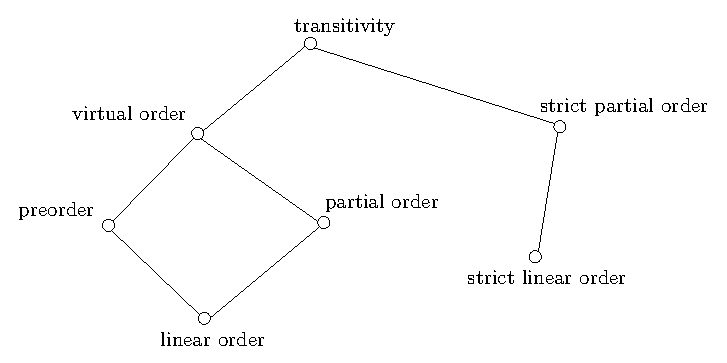
\includegraphics[height=50mm]{strukture-en.eps}
\end{center}

Hasse diagram

$R$ - relation that partially or strictly partially orders $S$

$xRy\cee $ we can get from $x$ to $y$ in the diagram moving only upwards

\bigskip
------------------------------------------------------------------------------

\bigskip

\textbf{ Example:} $A = \{1,2,3\}$, $S = {\cal P}(A)$, $R$: strict inclusion

\begin{center}
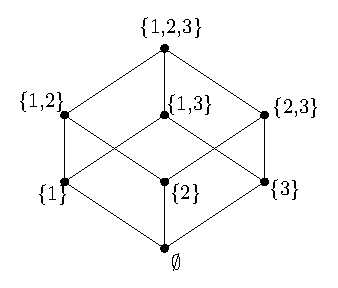
\includegraphics[height=40mm]{Hasse.eps}
\end{center}

\bigskip

------------------------------------------------------------------------------
\bigskip

\textbf{ Example:} Hasse diagram of a totally or strictly totally ordered set:

\begin{center}

\includegraphics[height=40mm]{Hasse1.eps}
\end{center}

\pagebreak
%lectures together with midterms
\subsection{Lattice}

A {\em lattice} structure is a partial order with particularly nice features.
In order to define it, we need some definitions.

\bigskip

Let a set $S$ be partially ordered with relation $R$ and let $U\subseteq S$.

If there exists $a\in S$ such that for all $x\in U$ it holds $aRx$, we say that
$a$ is an {\em $R$-lower bound} for $U$.

\bigskip
If there exists $b\in S$ such that for all $x\in U$ it holds $xRb$, we say that
$b$ is an {\em $R$-upper bound} for $U$.

\bigskip
If $U$ has an $R$-lower bound, we say that $U$ is {\em $R$-bounded from below}.

\bigskip
If $U$ has an $R$-upper bound, we say that $U$ is {\em $R$-bounded from above}.

\bigskip
If $U$ has an $R$-upper bound as well as an $R$-lower bound, we say that
$U$ is {\em $R$-bounded}.

\bigskip
$a\in S$ is an {\em $R$-greatest lower bound ($R$-infimum)} of a subset $U$
$\cee$ $a$ is an $R$-lower bound for $U$ and for every $R$-lower bound $x$ for $U$ it holds $xRa$.

Notation: $a = R$-$\inf U$.

\bigskip
$b\in S$ is an {\em $R$-least upper bound ($R$-supremum)} of a subset $U$
$\cee$ $b$ is an $R$-upper bound for $U$ and for every $R$-upper bound $x$ for $U$ it holds $bRx$.

Notation: $b = R$-$\sup U$.

\bigskip
Because of antisymmetry, every subset $U\subseteq S$ has at most one $R$-$\sup$
and at most one $R$-$\inf$.

But some subsets might have neither of them!

\bigskip
\textbf{ Example:}

$S = \mathbb{Q}$, $R = \le$

$$U = \{x~;~x\in \mathbb{Q}\inn 0\le x \inn x^2\le 2\}$$

Set $U$ is bounded from above and from below.

$\inf U = 0$, $\sup U$ does not exist!

\medskip
$$V = \{x~;~x\in \mathbb{Q}\inn 0\le x \inn 2\le x^2\le 5\}$$

Set $V$ is bounded, but neither $\inf V$ nor $\sup V$ exist.

\begin{definition}
Set $S$ has the structure of a {\em lattice} with respect to relation $R$ $\cee$
$R$ partially orders $S$ and every {\em two-element} subset $X\subseteq S$
has an $R$-supremum and an $R$-infimum.
\end{definition}

\textbf{Remark:} the structure of a lattice can be defined purely algebraically.

\subsubsection{Examples of lattices}
\begin{enumerate}
  \item $A$ - set

  ${\cal P}(A)$ -- power set

  ${\cal P}(A)$ is a lattice with respect to  $R = \subseteq$:
  \begin{itemize}
    \item partial order $\checkmark$
     \item $E,F\subseteq A$, $E\neq F$:

     $\inf\{E,F\} = E\cap F$

     $\sup\{E,F\} = E\cup F$
  \end{itemize}
  \item Let $R$ linearly order $S$.

  $a, b\in S, a\neq b\sledi aRb$ or $bRa$

$aRb\sledi R\textrm{-}\inf\{a,b\} = a,~R\textrm{-}\sup\{a,b\} = b$.

$bRa\sledi R\textrm{-}\inf\{a,b\} = b,~R\textrm{-}\sup\{a,b\} = a$.

  \item $S = \mathbb{N}\backslash \{0\}$, $R = |$ (relation  of divisibility).
  \begin{itemize}
    \item partial order $\checkmark$
    \item $x,y\in \mathbb{N}$, $x\neq y$

    $\inf\{x,y\} = $ greatest common divisor of $x$ and $y$

    $\sup\{x,y\} = $ least common multiple of $x$ and $y$
  \end{itemize}
\end{enumerate}



\begin{figure}[hb]
	\centering
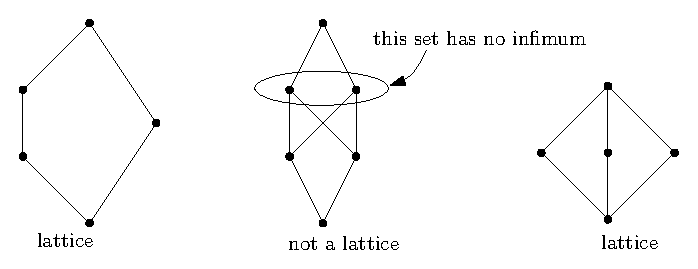
\includegraphics[height=40mm]{Hasse4-en.eps}
\caption{Some further examples with Hasse diagrams.}
\end{figure}

\pagebreak

In every lattice, every \underline{finite} non
empty subset of set $S$ has an infimum and a supremum!

\begin{proposition}
Let $S$ have the structure of a lattice with respect to $R$. Then for every three elements
$a_1,a_2,a_3\in S$, it holds that
$$R\textrm{-}\inf\{a_1,a_2,a_3\} = R\textrm{-}\inf\{R\textrm{-}\inf\{a_1,a_2\}, a_3\}\,.$$
\end{proposition}

\begin{proof}
Let $a = R\textrm{-}\inf\{R\textrm{-}\inf\{a_1,a_2\}, a_3\}$.

\emph{ $a$ is a lower bound of the set $\{a_1,a_2,a_3\}$:}

  $aRa_3$, since $a$ is a lower bound of the set $\{R\textrm{-}\inf\{a_1,a_2\}, a_3\}$.

  Similarly
   $aR(R\textrm{-}\inf\{a_1,a_2\})$, but since $(R\textrm{-}\inf\{a_1,a_2\})Ra_1$ and $R$ is transitive, we get $aRa_1$.
   Similarly we also get $aRa_2$.


\emph{ $a$ is the greatest lower bound of the set $\{a_1,a_2,a_3\}$:}

Let $x$ be an arbitrary lower bound of the set $\{a_1,a_2,a_3\}$. Therefore $xRa_1$, $xRa_2$ and $xRa_3$.

$xRa_1, xRa_2\sledi xR(R\textrm{-}\inf\{a_1,a_2\})$.

$xR(R\textrm{-}\inf\{a_1,a_2\}) \inn xRa_3\sledi xRa$.
\end{proof}

Similarly for supremum. We can repeat the procedure and show the existence of infimum and supremum for
arbitrary finite nonempty sets.

\medskip
%\textbf{ V razmislek:} Kako bi dokazali obstoj $R$-$\inf\{a_1,\ldots, a_n\}$?
%
%\medskip

\begin{corollary}
If $S$ is a lattice with respect to $R$, then every \underline{finite} nonempty set has both $R\textrm{-}\inf$
and $R\textrm{-}\sup$.
\end{corollary}

%(Proof: exercise.)

%\begin{proposition}
%Naj ima $S$ strukturo mreže glede na $R$. Tedaj za vsake tri elemente $a_1,a_2,a_3\in S$ velja
%$$R\textrm{-}\inf\{a_1,a_2,a_3\} = R\textrm{-}\inf\{R\textrm{-}\inf\{a_1,a_2\}, a_3\}\,.$$
%\end{proposition}
%
%\begin{proof}
%Let $a = R\textrm{-}\inf\{R\textrm{-}\inf\{a_1,a_2\}, a_3\}$.
%
%\emph{ $a$ je spodnja meja množice $\{a_1,a_2,a_3\}$:}
%
%  $aRa_3$, saj je $a$ spodnja meja množice $\{R\textrm{-}\inf\{a_1,a_2\}, a_3\}$.
%
%  Podobno je
%  $aR(R\textrm{-}\inf\{a_1,a_2\})$, ker pa je $(R\textrm{-}\inf\{a_1,a_2\})Ra_1$ and je $R$ transitive, je $aRa_1$. Podobno je tudi $aRa_2$.
%
%
%\emph{ $a$ je najveèja spodnja meja množice $\{a_1,a_2,a_3\}$:}
%
%Let $x$ poljubna spodnja meja množice $\{a_1,a_2,a_3\}$. Torej je $xRa_1$, $xRa_2$ and $xRa_3$.
%
%$xRa_1, xRa_2\sledi xR(R\textrm{-}\inf\{a_1,a_2\})$.
%
%$xR(R\textrm{-}\inf\{a_1,a_2\}) \inn xRa_3\sledi xRa$.
%\end{proof}
%
%Podobno za supremum. Postopek lahko ponavljamo and
%pokažemo obstoj infimuma and supremuma poljubne konène neprazne množice.

%\medskip
%\textbf{ V razmislek:} Kako bi dokazali obstoj $R$-$\inf\{a_1,\ldots, a_n\}$?

\medskip
%
%\begin{corollary}
%Èe je $S$ mreža glede na $R$, ima vsaka \underline{finite} neprazna set $R\textrm{-}\inf$
%and $R\textrm{-}\sup$.
%\end{corollary}
%
We may require the existence of infimum and supremum for \emph{ all} nonempty subsets (not only for finite ones):

\begin{definition}
Set $S$ has the structure of a {\em complete lattice} with respect to relation $R$ $\cee$
$R$ partially orders set $S$ and \underline{every} nonempty subset $X$ of set $S$ has $R$-inf and $R$-sup.
\end{definition}

Clearly, every complete lattice is also a lattice with respect to the same relation $R$.
Every finite lattice is a complete lattice.

\bigskip
\textbf{ Example:}

$A$ -- arbitrary set

${\cal P}(A)$ is a complete lattice for $\subseteq$:

If ${\cal A}$ is a nonempty family of subsets of set $A$, then
$$(\subseteq)\textrm{-}\inf {\cal A} = \cap {\cal A}$$
and
$$(\subseteq)\textrm{-}\sup {\cal A} = \cup {\cal A}\,.$$

\bigskip

\textbf{ Question:} Is the set ${\mathbb R}$ of real numbers a complete lattice with respect to relation ``$\le$''?

\bigskip

$\mathbb{R}$ is not a complete lattice with respect to $\le$:
the whole set $\mathbb{R}$ is not bounded! (it has neither a supremum nor an infimum)

We can extend the set of real numbers to a complete lattice by adding to it elements
$\infty$ and $-\infty$, and require $x\le \infty$ for all $x\in \mathbb R$ and $-\infty\le x$ for all $x\in \mathbb R$.


------------------------------

Hasse diagram of the $9$ order structures that we have seen:

\begin{center}
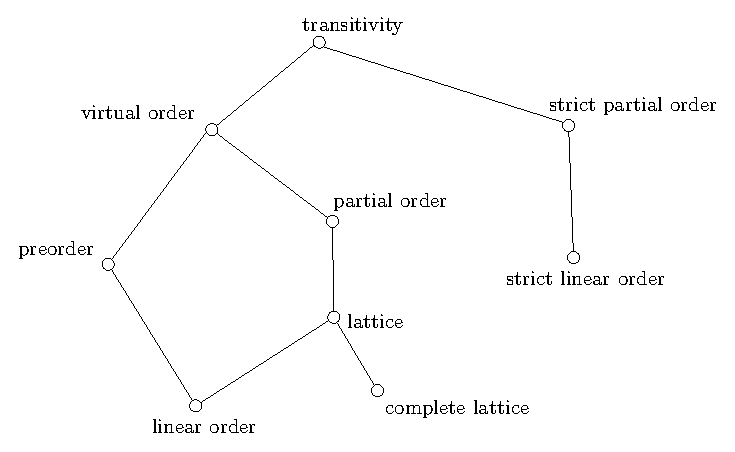
\includegraphics[height=70mm]{strukture2-en.eps}
\end{center}

$x$ is below  $y$ $\cee$ $x$ is a special case of $y$.

% 17. predavanje, 2 uri, 13. 12. 2011
%
%Ponovitev:
%\begin{itemize}
%\item Hassejev diagram struktur urejenosti:
%\begin{center}
%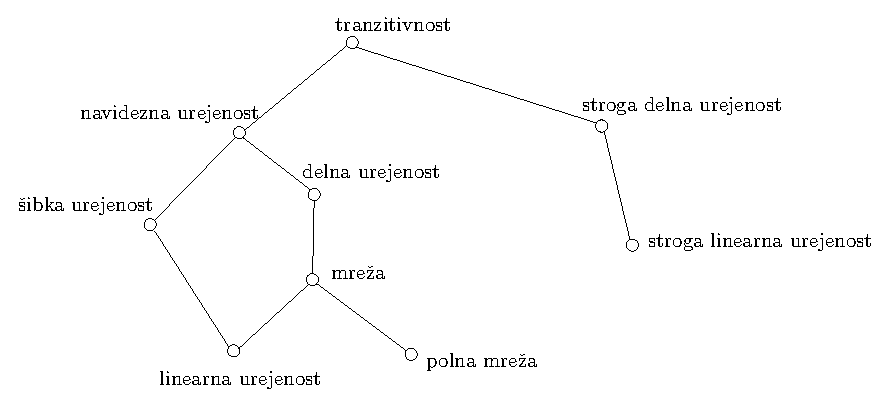
\includegraphics[height=70mm]{strukture3.eps}
%\end{center}
%
%$x$ je pod $y$ $\cee$ $x$ je poseben primer $y$.
%
%$R$ {\em strogo delno ureja} $S$ $\cee$ $R$ je transitive and asymmetric.
%
%$R$ {\em strogo linearno ureja} $S$ $\cee$ $R$ je transitive, asymmetric and sovisna.
%
%\bigskip
%
%  \item Mreža: delna urejenost, kjer ima vsaka dvoelementna podmnožica supremum and infimum.
%
%  Polna mreža: vsaka podmnožica ima supremum and infimum.
%



\appendix
\cleardoublepage\part*{Appendix}
\chapter{Additional Topics from Set Theory}
\section{Logical consequences}

We are given propositions $C_1,\ldots, C_m$, composed of propositions $A_1,\ldots, A_n$.
Let us determine all propositions $B$ for which $$C_1\inn\cdots\inn C_m\sledi B$$
is a tautology. Such a proposition $B$ is called  {\em logical consequence}
of propositions $C_1,\ldots, C_m$.

Special cases:
\begin{itemize}
  \item $C_1\inn\cdots\inn C_m$ tautology  $\sledi B$ tautology
  \item $C_1\inn\cdots\inn C_m$ contradiction $\sledi B$ any proposition
\end{itemize}

Otherwise, we take the following approach:

We express the proposition $C_1\inn\cdots\inn C_m$ in its canonical CNF.
$C_1\inn\cdots\inn C_m$ is the conjunction of a number of basic disjunctions (maxterms), composed of
propositions $A_1,\ldots, A_n$:
$$( \ali\ali\ali) \inn ( \ali\ali\ali) \inn \cdots \inn (\ali\ali\ali)$$

The following holds:

1. If $B$ is the conjunction of any number of these maxterms, then
$$C_1\inn\cdots\inn C_m\sledi B$$
is a tautology!

(Indeed: if proposition $C_1\inn\cdots\inn C_m$ is true, then all the maxterms appearing in the canonical CNF of it are true. Therefore also the conjunction of any number of these maxterms is true.)

2. If $C_1\inn\cdots\inn C_m\sledi B$ is a tautology, then the canonical CNF of $B$ can only contain those maxterms that also appear
in the canonical CNF of $C_1\inn\cdots\inn C_m$.

(Indeed: if, in the canonical CNF of $B$ we have a maxterm corresponding to a truth assignment $d$, which does not appear in the canonical CNF for
$C_1\inn\cdots\inn C_m$, then proposition $B$ is false at $d$, while proposition $C_1\inn\cdots\inn C_m$ is true at $d$. This is a contradiction with the assumption that  $C_1\inn\cdots\inn C_m\sledi B$ is a tautology.)

\bigskip
\textbf{ Example:}

$C_1$: A man speaks the truth or is not brave.

$C_2$: If a man is free, he is brave.

\medskip
$A_1$: A man speaks the truth.

$A_2$: A man is brave.

$A_3$: A man is free.

\medskip

$C_1: A_1\ali \neg A_2$

$C_2: A_3\sledi A_2$

$C_1\inn C_2: (A_1\ali \neg A_2) \inn (A_3\sledi A_2)$

\medskip
Truth table:

$$\begin{tabular}{c|c|c|c|c|c|c}
  \hline
  % after \\: \hline or \cline{col1-col2} \cline{col3-col4} ...
   & $A_1$ & $A_2$ & $A_3$ & $A_1\ali \neg A_2$ & $A_3\sledi A_2$ & $C_1\inn C_2$ \\
  \hline
  1. & 1 & 1 & 1 & 1 & 1 & 1 \\
  2. & 1 & 1 & 0 & 1 & 1 & 1 \\
  3. & 1 & 0 & 1 & 1 & 0 & 0 \\
  4. & 1 & 0 & 0 & 1 & 1 & 1 \\
  5. & 0 & 1 & 1 & 0 & 1 & 0 \\
  6. & 0 & 1 & 0 & 0 & 1 & 0 \\
  7. & 0 & 0 & 1 & 1 & 0 & 0 \\
  8. & 0 & 0 & 0 & 1 & 1 & 1 \\
\end{tabular}$$

Canonical CNF:
\begin{align*}
(\neg A_1\ali A_2\ali \neg A_3) & \inn (A_1\ali \neg A_2\ali \neg A_3)\\ 
& \inn (A_1\ali \neg A_2\ali A_3) \\
& \inn (A_1\ali A_2\ali \neg A_3)
\end{align*}
$$
$$

We can obtain all logical consequences that are not tautologies by choosing one or more maxterms and connecting them conjunctively.
The number of such consequences is
$${4\choose 1} + {4\choose 2} +{4\choose 3} + {4\choose 4}  = 4+6+4+1 = 15\,.$$

Let us analyze one of them:
$$(A_1\ali \neg A_2\ali \neg A_3) \inn (A_1\ali A_2\ali \neg A_3)$$
$$\cee$$
$$(A_1\ali \neg A_3 \ali\neg A_2) \inn (A_1\ali \neg A_3\ali A_2)$$
$$\cee$$
$$((A_1\ali \neg A_3) \ali\neg A_2) \inn ((A_1\ali \neg A_3)\ali A_2)$$
$$\cee$$
$$(A_1\ali \neg A_3)\ali (\neg A_2\inn A_2)$$
$$\cee$$
$$A_1\ali \neg A_3$$
The proposition reads: {\em A man speaks the truth or is not free.}

\bigskip

Suppose also that somebody asks us: Is proposition $A_1$ a tautological consequence of propositions $C_1$ and $C_2$?

In this case, we express proposition $A_1$ in its canonical CNF with respect to the atomic propositions $A_1$, $A_2$, $A_3$:

Applying implication (18) twice, we can write $A_1$ as
$$A_1\ali (A_2\inn \neg A_2)\ali (A_3\inn \neg A_3)\,.$$
Applying distributivity, we obtain the canonical CNF of $A_1$:
\begin{align*}
    (A_1\ali A_2\ali A_3)
    & \inn (A_1\ali A_2\ali \neg A_3)\\
    & \inn (A_1\ali \neg A_2\ali A_3)
    \inn (A_1\ali \neg A_2\ali \neg A_3)\,.
\end{align*}
We notice that disjunction $A_1\ali A_2\ali A_3$ does not appear in the canonical CNF of proposition $C_1\inn C_2$.
Therefore, the answer to the above question is: no. \qed

% 7. predavanje, 60', 25. 10. 2012

\section{Inference}

Facts:
\begin{itemize}
  \item I will go to the match.
  \item In the evening, I will do the homework.
  \item If I go to the match and then to the cinema, I will not have the time to do the homework.
\end{itemize}
Can I infer that I will not be able to go to the cinema?

\medskip
\textbf{ Solution:}

Let us define the following propositions:

$A_1$: I will go to the match.

$A_2$: In the evening, I will do the homework.

$A_3$: I will go to the cinema.

$C_1$: $A_1$

$C_2$: $A_2$

$C_3$: $A_1\inn A_3\sledi \neg A_2$.

We have to determine whether the implication
$$C_1\inn C_2\inn C_3\sledi \neg A_3$$
is a tautology.


Suppose this is not the case: let $d$ be a truth assignment for which the antecedent
$C_1\inn C_2\inn C_3$ is true,
while the consequent $\neg A_3$ is false.
Since the consequent $\neg A_3(d)$ is false, the proposition $A_3(d)$ is true.

Since the antecedent $C_1\inn C_2\inn C_3$ is true, both propositions $C_1=A_1$ and $C_2=A_2$ are true for assignment $d$.
What is the value of $C_3$, that is,~$A_1\inn A_3\sledi \neg A_2$?
Proposition $A_1\inn A_3$ is true at assignment $d$, while proposition $\neg A_2$ is false. Therefore, also proposition $C_3$ is false.
However this is a contradiction with the assumption that the conjunction
$C_1\inn C_2\inn C_3$ (antecedent) is true.

This contradiction shows that the implication
$$C_1\inn C_2\inn C_3\sledi \neg A_3$$
is indeed a tautology, hence the above inference is correct. (I will not make it to the cinema.)
\qed

\bigskip

The following facts are given:
\begin{itemize}
  \item This bird is not a bird, or it has wings.
  \item If this animal is a bird, then it lays eggs.
\end{itemize}
Is the following inference correct?
{\em If this animal does not have wings, then it does not lay eggs.}

\medskip
\textbf{ Solution:}

Let us define the following propositions:

$A_1$: This animal is a bird.

$A_2$: This animal has wings.

$A_3$: This animal lays eggs.

$C_1$: $\neg A_1\ali A_2$

$C_2$: $A_1\sledi A_3$

$B$: $\neg A_2\sledi \neg A_3$.

We have to determine whether the implication
$$C_1\inn C_2\sledi B$$
is a tautology.

So let us suppose that it is not: let $d$ be a truth assignment at which the antecedens
$C_1\inn C_2$ is true and the consequent $B$ is false.
Since the consequent $B(d)$ is false, the proposition $\neg A_2(d)$ is true, and the proposition
$\neg A_3 (d)$ is false. It follows that the proposition $A_2(d)$ is false, and the proposition
$A_3(d)$ is true.

Since the antecedens $C_1\inn C_2$ is true at the truth assignment $d$, also the proposition $C_1$ is true at $d$: $\neg A_1\ali A_2$.
However since the proposition $A_2(d)$ is false, the proposition
$\neg A_1(d)$ must be correct. Equivalently: proposition $A_1$ is false at truth assignemnt $d$.

The truth assignment is already completely determined with this: $A_1(d)$ and $A_2(d)$ are false propositions, and
$A_3(d)$ is true. We can check that also the proposition $C_2$ is correct at this truth assignment.

We have not reached a contradiction, we constructed a truth assignment, for which the proposition $$C_1\inn C_2\sledi B$$
is flase. (This happens only in the case when {\em this animal is not a bird, it has no wings, and lays eggs.})
\qed

\medskip
\begin{sloppypar}
{\em The above examples nicely illustrate that the process of proving that a particular proposition is a tautology is  the same as the process of proving  that the a certain proposition is not a tautology. In both cases, we are trying to construct a truth assignment $d$, for which the proposition is false.
If we do that, then we have a proof that the proposition is not a tautology. If we get a contradiction, we have thus proved that the proposition is a tautology!}
\end{sloppypar}

\bigskip
\textbf{ Homework:}
Found out whether the following inference is correct.

Facts:

Duke was killed by one of his staff: the cook, the servant or the driver.

If the killer was the cook, she poisoned the food.

If the killer was the driver, he put a bomb in the car.

The food was not poisoned and the servant is not a murderer.

Conclusion: The killer was the driver.
	content...

\chapter{Additional Topics from Set Theory}

\section{On Axioms}

Every mathematical theory is based on a set of axioms --- basic propositions that we {\ em assume} to be correct.
These axioms define the basic properties that objects of a certain theory should satisfy (e.g.~integers, real numbers, groups, vector spaces, graphs, manifolds, ...). From the axioms new truths (claims, consequences, theorems ...) are derived by logical reasoning.

In Set Theory, the situation is the same! There are several families of axioms, but the most established are seven particular axioms, called {\em axioms of ZFC} (Zermelo - Fraenkel - (Axiom of) Choice).

These axioms ensure the existence of sets and ways of forming new sets from existing ones.
Except for the Axiom of Choice, which is of special interest, we will not discuss other axioms here in detail.

To understand why we need the axioms, let's see why the set of all sets does not exist!

\subsection*{Russell's Antinomy}

We can form very big sets of sets (or families of sets), see the example below

\paragraph{Example.}  $\mathbb{Q}$: The set of rational numbers is a set of sets:
$$0,5 = \left\{\frac{1}{2}, \frac{2}{4}, \frac{3}{6}, \cdots\right\}$$
(Fraction is understood as an ordered pair of integers. Ordered pair $ (a, b) $ can be defined as the set $\{\{a \}, \{a, b \} \} $.)

This gives the following question:
\subsection*{Is there a {\em set of all sets?}}

We will prove, by contradiction that there is no such set!

So suppose there is. Let $ A $ be the set of all sets.
For each set, we can ask whether it contains itself as an element. $\mathbb{N} $ is not an element of itself!
The set of all abstract notions has itself as an element.

Let $B \subseteq A $ be that subset of $A$ that has for elements precisely those sets from $A$ that do not contain themselves as elements.
Does the set $B$ contain itself as an element?

If yes, then it does not contain itself as an element!

What if $ B $ does not contain itself as an element? Then, by definition, $ B \in B $, a contradiction.

{\em The set of all sets does not exist!}

{\centerline \em Nothing contains everything.}

$$ \textit{(mathematical) space does not exist.}$$

So, in forming new sets we should not trust too much our intuition ...
Axioms are needed to ensure the existence of certain sets (e.g.~the axiom of pairs, the axiom of subsets).

\section{Axioms of Zermelo-Fraenkel set theory}

\begin{enumerate}
	\item Axiom of extensionality (set equality)
	$$\forall A\, \forall B\, (\forall x \,(x\in A \cee x\in B) \sledi A = B)$$
	
	\item Axiom of an empty set:
	{\emph There is an empty set.}
	$$\exists B\, \forall x\, (x\not \in B)$$
	
	\item Axiom of pairing: {\emph Any couple of elements from universe may form a 2-set.}
	$$\forall u\, \forall v\, \exists B\, \forall x\, (x\in B \cee x = u\textrm{ ali }x = v)$$
	
	\item Axiom of union: {\emph The union over the elements of a set exists. }
	$$\forall A\, \exists B\, \forall x\, (x\in B \cee (\exists b\in A) x\in b)$$
	
	\item Axiom of power set: {\emph For each set, the set of all its subsets exists.}
	$$\forall a\, \exists B\, \forall x (x\in B \cee x\subseteq a)$$
	
	\item Axiom schema of specification: {\emph  The set builder notation makes sense!}
	
	For each logical predicate $\varphi$ which include variables $t_1,\ldots, t_k$, but not  $B$, we have:
	$$\forall t_1\,\cdots\, \forall t_k\,\forall c\,\exists B \,\forall x \,(x\in B \cee x\in c \inn \varphi)$$
	
	\paragraph{Example.}
	(Fpr $k = 1$):
	
	$\forall a \,\forall c \,\exists B \, \forall x\, (x\in B \cee x\in c \inn x\in a)$
	
	This means in particular that for each sets $a$ and $c$ there is a set  $B = a\cap c$, i.e. their intersection.
	
	\medskip
	As a result of this axiom, the set builder notation is always well-defined, i.e. we may define sets as
	$$\{x\in A; P(x)\}\,.$$
	
	\paragraph{Example.} $\{x\in \mathbb{R}; x\ge 0\}$.
	
	\item Axiom of infinity: {\emph There exists an infinite set.}
	$$\exists A\,(\emptyset \,\in A \inn (\forall a\in A)\, (a\cup \{a\}\in A))$$
	

	
	\item Axiom schema of replacement: {\emph The image of a set under any definable function will also fall inside a set.}
	
	This schema allows us to describe functions in a form
	$$\{f(x); x\in A\}\,,$$
	where $f$ is any function with a domain which contains $A$.
	
	\paragraph{Example.} We may write a set $\{x^2; x\in \mathbb{R}\}$. This is equal to $\{x\in \mathbb{R}; x\ge 0\}$.
	
	%Za vsako formulo $\varphi(x,y)$, ki ne vsebuje ?rke $B$,
	%je naslednji izraz aksiom:
	%$$\forall t_1\,\cdots \forall t_k\,\forall A\,[(\forall x\in A)\,\forall y_1\, \forall y_2\, (\varphi(x,y_1) \inn \varphi(x,y_2) \sledi y_1 = y_2)$$
	%$$\sledi \exists B\, \forall y\, [y\in B \cee (\exists x\in A)\,\varphi(x,y)]$$
	
	\item Axion of regularity: {\emph Every non-empty set x contains a member y such that x and y are disjoint sets.}
	$$(\forall A\neq \emptyset)\,(\exists m\in A)\,(m\cap A = \emptyset)$$
	
	This implies, for example, that for any $A$ and $B$,  niether $A\in B$ or $B\in A$.


	\item Axiom of choice: {\emph Each relation admits a function with the same domain.}
	$$(\forall \textrm{ relacijo }R)(\exists \textrm{ funkcija }F)(F\subseteq R \inn {\cal D}(F) = {\cal D}(R))$$
	We will cover this axiom in detail later, at the end of the Relations chapter.
\end{enumerate}
\noindent Some of above axioms maybe derived from the remaining ones, in particular 2., 3.~and 6.

\end{document}